\section{Alpha Energy and Spectral Shape}
\subsection{Observations}\label{ssec:E_obs}
In the energy spectra for each data set, it can be seen that for large-magnitude radii, compared to source-free runs, there is an excess of events falling in a Gaussian peak, as in the examples in Fig~\ref{fig:Epeaks}. The energy and width of the peak varies with radius. For positions with radii larger than 6.75\,mm in magnitude, the mean alpha energy is larger than 2614\,keV, limiting the gamma-interaction background contribution in the peak region. See Figs.~\ref{fig:Efit_110} and~\ref{fig:Efit_360} for several examples. Therefore, despite the low alpha interaction rate, the peak can be clearly identified and fit.

A tail of events at low energy is expected to occur along with the peak, due to variation in the alpha penetration depth. However, in practice, adding an exponentially modified Gaussian component to the peak fitting function does not improve the goodness of fit. The low alpha rate and large standard deviation of the Gaussian peak often lead the preferred fit of the tail function to accommodate the background, rather than improving the fit to the peak. 

In the fit, the background is modeled by a linear function, which accounts for the gamma pile-up and muon background remaining after muon veto, single-site, and pile-up cuts. No other event cuts are used to produce these spectra. The results of these fits are shown in Figs~\ref{fig:Efit_mu} and ~\ref{fig:Efit_sig}.

\begin{figure*}[]
 \centering
  \begin{subfigure}[t]{.45\textwidth}
 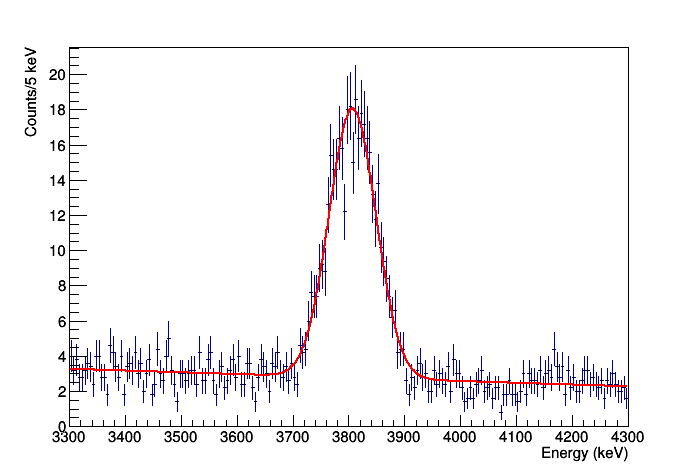
\includegraphics[width=1.0\columnwidth]{/Users/jgruszko/Documents/Thesis/Plots/Ch6/DS110_0_Efit.png}
  \caption{The energy spectrum of a data set taken at 11 turns ($r= -13.5$\,mm), a total of 25.1\,hrs of runtime.}
 \label{fig:Efit_110}
\end{subfigure}
\hfill
  \begin{subfigure}[t]{.45\textwidth}
 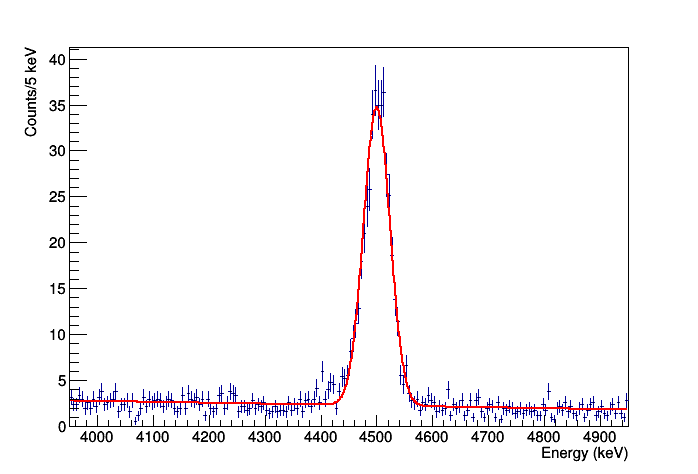
\includegraphics[width=1.0\columnwidth]{/Users/jgruszko/Documents/Thesis/Plots/Ch6/DS360_2_Efit.png}
  \caption{The energy spectrum of a data set taken at 36 turns ($r = 24$\,mm), with 30.1\,hrs of runtime.}
 \label{fig:Efit_360}
\end{subfigure}
\hfill
 \begin{subfigure}[t]{.45\textwidth}
 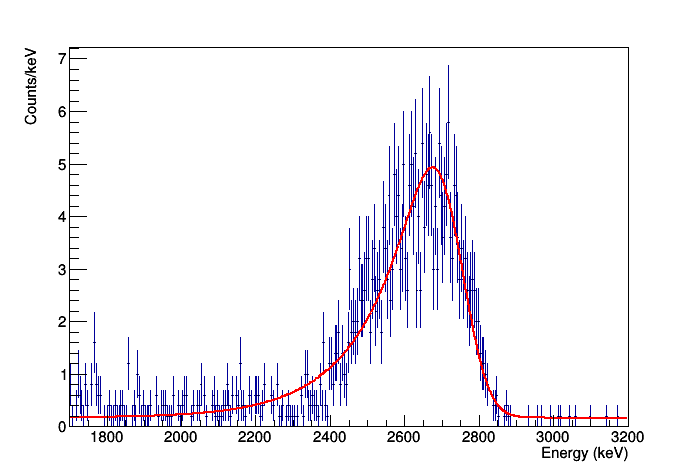
\includegraphics[width=1.0\columnwidth]{/Users/jgruszko/Documents/Thesis/Plots/Ch6/DS170_0_Efit.png}
  \caption{The energy spectrum of a data set taken at 17 turns ($r = -4.5$\,mm), a total of 19.1\,hrs of runtime, with a cut selecting near-point-contact events (${\tt aenorm} > 1.5$). At small radii ($r<6$\,mm), the peaks become highly non-Gaussian, and the fit is dominated by the low-energy tail. In addition to the fit results in Table~\ref{tab:Efits_aecut}, energy ranges for these small-radius positions are given in Table~\ref{tab:E_ranges}.}
 \label{fig:Efit_170}
\end{subfigure}
\hfill
 \begin{subfigure}[t]{.45\textwidth}
 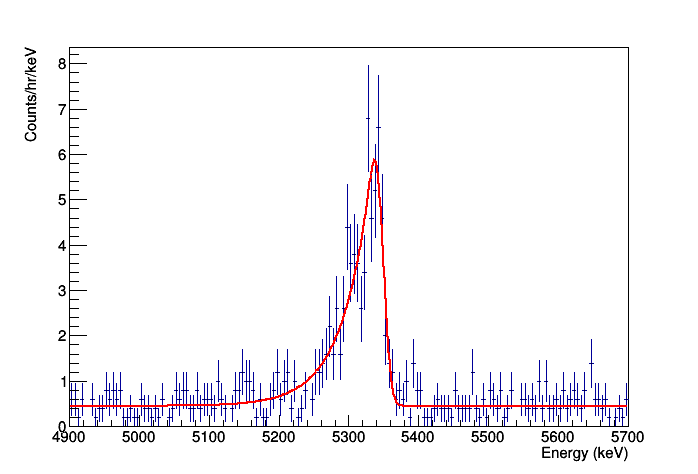
\includegraphics[width=1.0\columnwidth]{/Users/jgruszko/Documents/Thesis/Plots/Ch6/DS195_all_hiEfit.png}
 \caption{The sum energy spectrum of all runs taken at 19.5 turns ($r = -0.75$\,mm), a total of 82.4\,hrs of runtime, with a cut selecting near-point-contact events (${\tt aenorm} > 1.5$). Alphas incident on the point-contact have nearly the full incident energy, a narrower peak width, and visible low-energy tailing due to charge loss in the dead layer of the point-contact. Fit results are given in Table~\ref{tab:fullE_fitRes}.}
 \label{fig:Efit_195}
\end{subfigure}
 \caption{The energy spectra and peak fits for various scanning positions.} 
 \label{fig:Epeaks}
\end{figure*}

At radii smaller than 6\,mm, the alpha peak falls in a region of high gamma backgrounds. Due to the low alpha rate, it can not be fit without applying a pulse-shape cut to select the source events. A cut of ${\tt aenorm} >1.5$ selects near-point contact events while rejecting 99.8\% of background events. When this cut is applied, the remaining peak is highly non-Gaussian, as in Fig.~\ref{fig:Efit_170}. In these peaks, there is significant low-energy tailing, and the exponentially-modified Gaussian is included in the fit. The results of the fits are given in Table~\ref{tab:Efits_aecut}, where $\frac{1}{\tau}$ is the relaxation length (in keV) and  f$_{\tau}$ is the fractional contribution of the low-energy tail component to the peak area.

%\input{Efits.txt}

\begin{table*}[]
\begin{center}
\begin{tabular}{l l r r r r r}
Data Set & $\alpha$ Pos. (mm) & $\mu$ (keV) & $\sigma$ (keV) & f$_{\tau}$ & $\tau$ (keV$^{-1}$)& $\chi^2/N_{df}$ \\  \hline
{\tt DS170} & -4.5 & 2741$\pm$39 & 59$\pm$6 & 1.0$\pm$0.7 & 147$\pm$15 & 453/294 \\
{\tt DS180} & -3.0 & 2436$\pm$9 & 56$\pm$7 & 1.00$\pm$0.01 & 607$\pm$43 & 282/264 \\
\end{tabular}
\caption[The results of fits to the alpha energy peak at low-magnitude scanning radii]{The results of a Gaussian+low energy tail peak shape fit to the energy of alphas incident at small radii. A cut selecting near-point-contact events (${\tt aenorm} > 1.5$) is used to reduce the gamma background rate.} \label{tab:Efits_aecut}
\end{center}
\end{table*}

Due to the significant low-energy tail at these small radii, the Gaussian peak width does not give an accurate energy range for the alpha events observed. For the smallest radii ($r<3$\,mm), the Gaussian+tail model fit fails completely. For these data sets, we have given the estimated energy range of the observed alpha events, in Table ~\ref{tab:E_ranges}, either in lieu of or to supplement the description of the alpha energy spectra given by the fit results. These ranges were determined by eye-- they are the upper and lower energy bounds of the contiguous overdense region of high-A/E events that appear in the alpha-source runs, as in the boxed region of Fig.~\ref{fig:AEvE}.

\begin{table}[]
\begin{center}
\begin{tabular}{l l r r}
Data Set& $\alpha$ Pos. (mm) & $E_{min}$ (keV) & $E_{max}$ (keV) \\  \hline
{\tt DS170} & -4.5 & 2300 & 2850 \\
{\tt DS180} & -3.0 & 1200 & 2600 \\
{\tt DS185} & -2.25 & 700 & 2600 \\
{\tt DS190} & -1.5 & 800 & 2800 \\
\end{tabular}
\caption[Estimated energy ranges of alpha interactions at small-magnitude radii]{Estimated energy range of alpha interactions for source scans at small radii. At these positions, the peak is highly non-Gaussian. All data sets taken at each position are combined to determine these results.} \label{tab:E_ranges}
\end{center}
\end{table}

\begin{figure*}[]
 \centering
 \begin{subfigure}[]{.45\textwidth}
 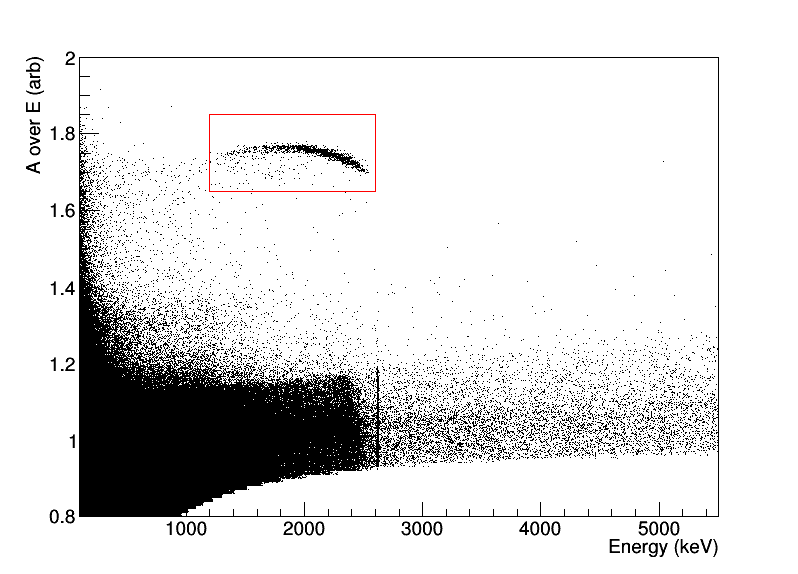
\includegraphics[width=1.0\columnwidth]{/Users/jgruszko/Documents/Thesis/Plots/Ch6/DS180_AE_all_wBox.png}
\end{subfigure}
 \begin{subfigure}[]{.45\textwidth}
 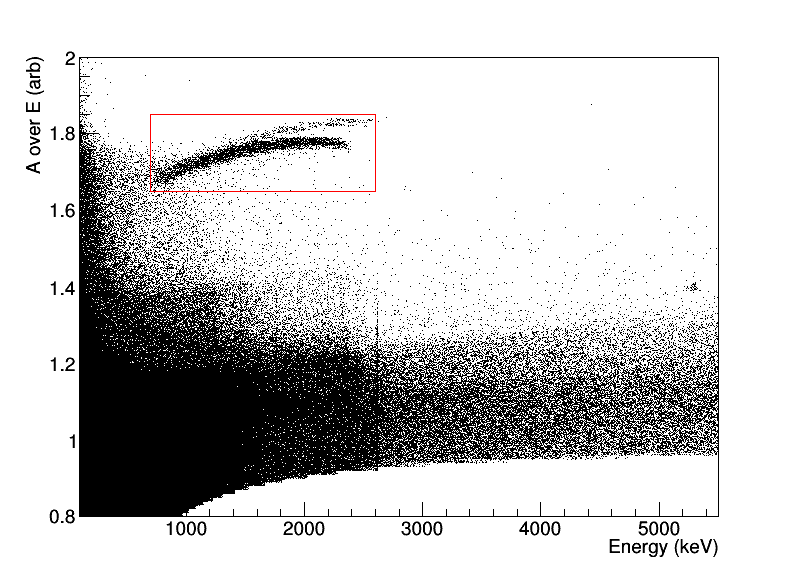
\includegraphics[width=1.0\columnwidth]{/Users/jgruszko/Documents/Thesis/Plots/Ch6/DS185_AE_all_wBox.png}
\end{subfigure}
 \caption[Plots of A/E vs. E for small-magnitude radii scans.]{At small radii, ({\it left:} $r=-3.0$\,mm, {\it right:} $r=-2.25$\,mm) the alpha peak becomes highly non-Gaussian and becomes impossible to fit with a Gaussian+low energy tail model. Depending on the scanning position, the energy ranges of the high-A/E alpha events (indicated by the boxed regions above and listed in Table~\ref{tab:E_ranges}) are given to supplement or stand in place of the fit result information.} 
 \label{fig:AEvE}
\end{figure*}

At scanning positions that are partially or entirely incident on the point-contact, an additional alpha peak in the spectrum appears at nearly the full energy of the emitted alpha. Again, an A/E cut selecting near-point-contact events ($A/E>1.5$) is applied to reduce the muon background. The peak shape is well-approximated by the sum of a Gaussian and an exponentially-modified Gaussian, as is expected from energy loss in the point-contact itself. See Fig~\ref{fig:Efit_195}. The results of these fits are given in Table~\ref{tab:fullE_fitRes}, . In {\tt DS195}, the source beam is entirely incident upon the point-contact, instead of being partially incident on the passivated surface. In this data set, the mean of the Gaussian component of the alpha peak falls at 5345\,keV, 141\,keV below the full 5.486\,MeV alpha energy. 

All of the peak energies of the fits to the alpha energy spectra are depicted in Fig.~\ref{fig:Efit_mu}, and the standard deviations of the gaussian components are depicted in Fig.~\ref{fig:Efit_sig}. Plotting these results as a function of the magnitude of the radius, as in Fig.~\ref{fig:Efit_rMag}, the results at the positive- and negative-radii scanning positions appear to be consistent. 

\begin{figure*}[]
 \centering
  \begin{subfigure}[]{\textwidth}
  \centering
 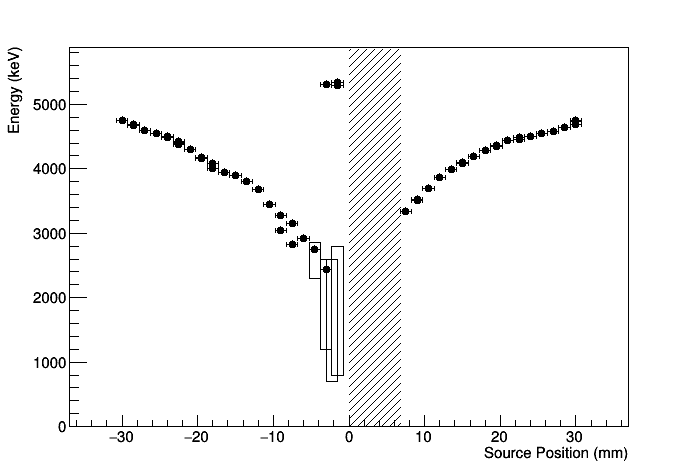
\includegraphics[height=3in]{/Users/jgruszko/Documents/Thesis/Plots/Ch6/EvR_wBoxes.png}
 \caption[The centroids of the alpha energy peaks in each data set]{The centroids of the alpha energy peaks in each data set. For scanning positions with significant low-energy tailing, the black box depicts the estimated full energy range of alpha events, as given in Table~\ref{tab:E_ranges}. At positions that are partially or completely incident on the point-contact, an additional peak appears at nearly the full incident alpha energy. } 
 \label{fig:Efit_mu}
\end{subfigure}
~
\begin{subfigure}[]{\textwidth}
\centering
 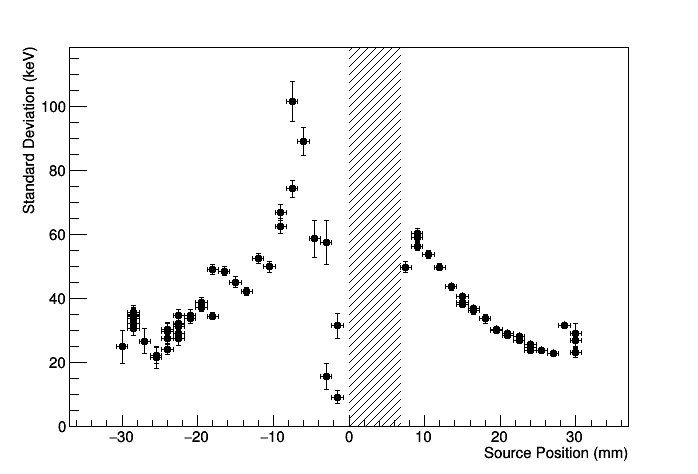
\includegraphics[height=3in]{/Users/jgruszko/Documents/Thesis/Plots/Ch6/EsigvR_wBoxes.png}
 \caption{The standard deviation of the gaussian component of the alpha energy peaks in each data set.} 
 \label{fig:Efit_sig}
 \end{subfigure}
 \caption[The results of Gaussian fits to the alpha energy peaks]{The results of Gaussian fits to the alpha energy peaks. The hashed box indicates the region on the detector surface that is obscured by the contact pin and contact pin support.}
\end{figure*}

\begin{figure*}[]
 \centering
 \begin{subfigure}[]{\textwidth}
 \centering
 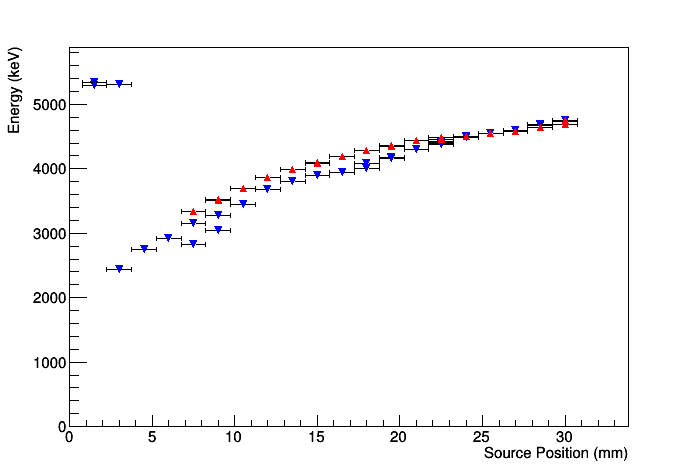
\includegraphics[height=3in]{/Users/jgruszko/Documents/Thesis/Plots/Ch6/EvRmag.png}
\end{subfigure}
 \begin{subfigure}[]{\textwidth}
 \centering
 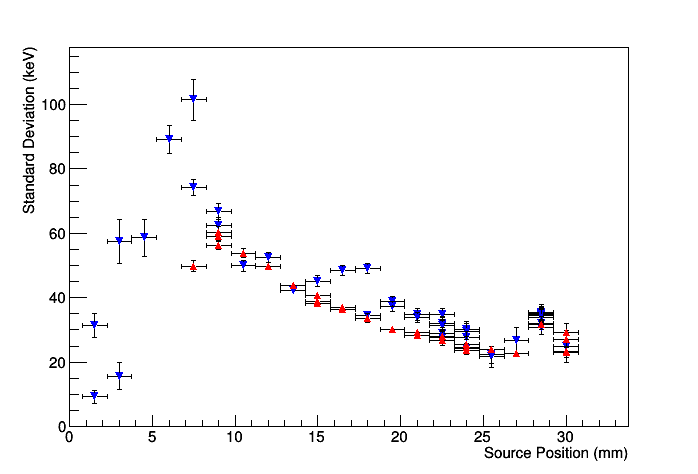
\includegraphics[height=3in]{/Users/jgruszko/Documents/Thesis/Plots/Ch6/EsigvRmag.png}
\end{subfigure}
 \caption[Energy fit results as a function of distance from the point contact]{The centroids {\it (top)} and standard deviations {\it (bottom)} of the alpha energy peaks in each data set, given as a function of the radial distract from the point contact. Negative-radius source positions appear as blue downward-pointing triangles, and positive-radius positions as red upward-pointing triangles. The results of the 0$\degree$ and 180$\degree$ scans appear to be consistent.} 
 \label{fig:Efit_rMag}
\end{figure*}

\begin{table*}[]
\begin{center}
\begin{tabular}{l l r r r r r}
Data Set & $\alpha$ Pos. (mm) & $\mu$ (keV) & $\sigma$ (keV) & f$_{\tau}$ & $\tau$ (keV$^{-1}$)& $\chi^2/N_{df}$ \\  \hline
{\tt DS185} & -2.25 & 5303$\pm$8 & 16$\pm$4 & 1.0$\pm$.9 & 12$\pm$11 & 314/274 \\
{\tt DS190} & -1.5 & 5298$\pm$5 & 31$\pm$4 & 0.3$\pm$.2 & 31$\pm$4 & 332/274 \\
{\tt DS195} & -0.75 & 5345$\pm$4 & 9$\pm$2 & 0.9$\pm$.1 & 41$\pm$6 & 335/274 \\
\end{tabular}
\caption[The results of fits to the alpha energy peak for events occurring in the point contact]{The results of a Gaussian+low energy tail peak shape fit to the energy of alphas incident on the point-contact. All data sets taken at each position are combined to determine these results.} \label{tab:fullE_fitRes}
\end{center}
\end{table*}

\subsection{Radial Dependence of Energy}\label{sssec:spec_fit}
Using the mean energies at each position found in Sec.~\ref{ssec:E_obs}, a spectral model describing the energy contributions of alpha contamination at a given position on the passivated surface can be constructed. Though it is slightly unnatural to consider the radial dependence of the energy, rather than the inverse, it will simplify the derivation of a full alpha energy spectrum for a given radial contamination model. Therefore we proceed with the former.

\begin{figure}[]
 \centering
 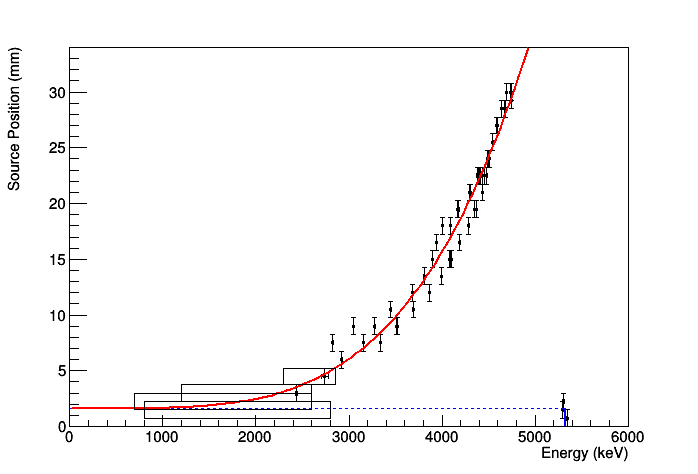
\includegraphics[width=1.\columnwidth]{/Users/jgruszko/Documents/Thesis/Plots/Ch6/RvsE_fit_wBoxes.png}
 \caption[A polynomial fit describing the radial dependence on energy]{Radii of the source incidence position, plotted with respect to the energy of the resulting alpha peak. Only data sets for which a gaussian (or gaussian+low-energy tail) peak shape modeled the alpha peak are included in the fit. The boxes represent the range of energies for the data sets that could not be fit, given in Table~\ref{tab:E_ranges}. The passivated-surface radii (scans with $r\geq3$\,mm), are fit with a fourth-order polynomial in energy (in red), and the energies of the point-contact positions are averaged (in blue).} 
 \label{fig:RvsE_fit}
\end{figure}

Plotting the radii of the measurements in which the source was incident on the passivated surface with respect to the centroid energies found at those radii, as in Fig.~\ref{fig:RvsE_fit}, and fitting to the fourth-order polynomial
$$ r = aE^4 + 1.6 $$
where $r$ is the source position radius, in mm, and $E$ is the energy of the resulting event, we find that the fit parameter $a = 5.50E-14\pm3E-16$, and the $\chi^2/N_{df}$ of the fit is 2.50.

The constant component is set to be 1.6\,mm because this is the outer radius of the point-contact of PONaMa-1; the passivated surface energy function should not exhibit a radial dependence below this value. When the constant component is allowed to float in the fit, it fits to a value of $1.4\pm.2$\,mm, consistent with a radius of 1.6\,mm. Therefore, we fix this parameter to the model-driven value. 

The choice of a fourth order polynomial was entirely driven by the observed spectral shape, and is not driven by any theoretical model. The goodness-of-fit is not improved by the addition of a quadratic component to the fitting function. If the polynomial of the fit is allowed to float, it fits to a value of $4.2\pm0.1$, and the $\chi^2/N_{df}$ of the fit is 2.44, only slightly improved from its previous value. Therefore, for the sake of simplicity, we fix the exponent to a value of 4.  

Though the energy spans of events at the lowest scanning radii (where a peak could not be fit to the spectrum) were not included in the fit, their range of values roughly agrees with those given by the fitting function. The increase in the width of the energy peak at low radii found from the derived spectral shape is not as dramatic as that seen in the data; if they matched, the red fit line in Fig.~\ref{fig:RvsE_fit} would traverse the full length (in the energy-axis) of each box. This, and the imperfect goodness-of-fit, indicates that there is additional energy-broadening that is not captured by the derived spectral shape function. However, this simple function appropriately captures most of the relevant energy information. 

To model the energies of alpha events on the point contact itself (at $r<1.6$\,mm), the mean energies of the 3 fits to the point-contact alpha peaks are averaged. Their average energy is $5323\pm3$\,keV. The energy at these radii is assumed to be independent of radius. 

\subsection{Discussion}
The energy of alpha events from the collimated source incident on the passivated surface of the detector is degraded at all radii, and is reduced far beyond the expected energy loss to a thin dead layer. Furthermore, the energy varies by up to a factor of 5 with the incident radius of the source. 

Both of these observations indicate that charge loss, whether to slow surface charge collection, charge trapping, or a combination of the two factors, is occurring. Additionally, the radial dependence of energy indicates that positive and negative charge carrier contributions are affected differently, as would be expected from their differing mobilities in germanium.

At positions near the point-contact of the detector, the relative contributions of electrons and electron-holes vary drastically over small distances. For instance, at radii less than 5\,mm, the weighting potential at the passivated surface of a detector similar to PONaMA-1 (see Fig.~\ref{fig:wp_z0}) varies by over 15\% over the diameter of the alpha source beam (1.75\,mm). At radii larger than 10\,mm, on the other hand, the weighting potential varies by less than 3\% over the diameter of the alpha source beam. 

Based on this difference in the weighting potential, the observed variation in the alpha source spectral peak shape is not unexpected. 

The weighting potential also allows us to infer that both positive and negative charges must be affected by the charge loss mechanism in the detector. If only the energy of the electrons were being lost, the alpha peak energy would be reduced by at most 10\% at radii larger than 13\,mm. Instead, we see, in Fig.~\ref{fig:Efit_mu}, the energy is reduced by up to 31\% of the full incident alpha energy for these radii. Overall, the energy dependence on radius is larger (steeper?) than the radial dependence of the weighting potential for all radii, with a difference that is particularly dramatic for large radii. 

If, instead, only the energy from the electron-holes were being affected, we would except the energy of the alpha peak to increase dramatically at radii less than 5\,mm. This is also not observed; the alpha peak falls steeply until the source beam is incident on the point contact itself, with peak energies below 50\% of the full alpha energy. 

Therefore, we must conclude that both positive and negative charges are being trapped and/or slowed for interactions near the passivated surface, regardless of the radial position of the interaction. Conclusions concerning possible charge-loss mechanisms are discussed in Sec.~\ref{sec:models}.

Events incident on the p-contact, on the other hand, do not show indications of significant charge-trapping. The average energy loss observed is consistent with the loss seen in scans of the point contact of BEGe-type PPC detectors \cite{Agostini_thesis}. In that work, the energy loss was found to indicate a dead layer thickness of $519\pm15$\,nm, larger than the manufacturer-cited Boron implantation depth of approximately 300\,nm. This could indicate the presence of additional material on the surface of the point-contact or deadness extending beyond the cited boron-implantation depth. 

\begin{figure}[]
 \centering
 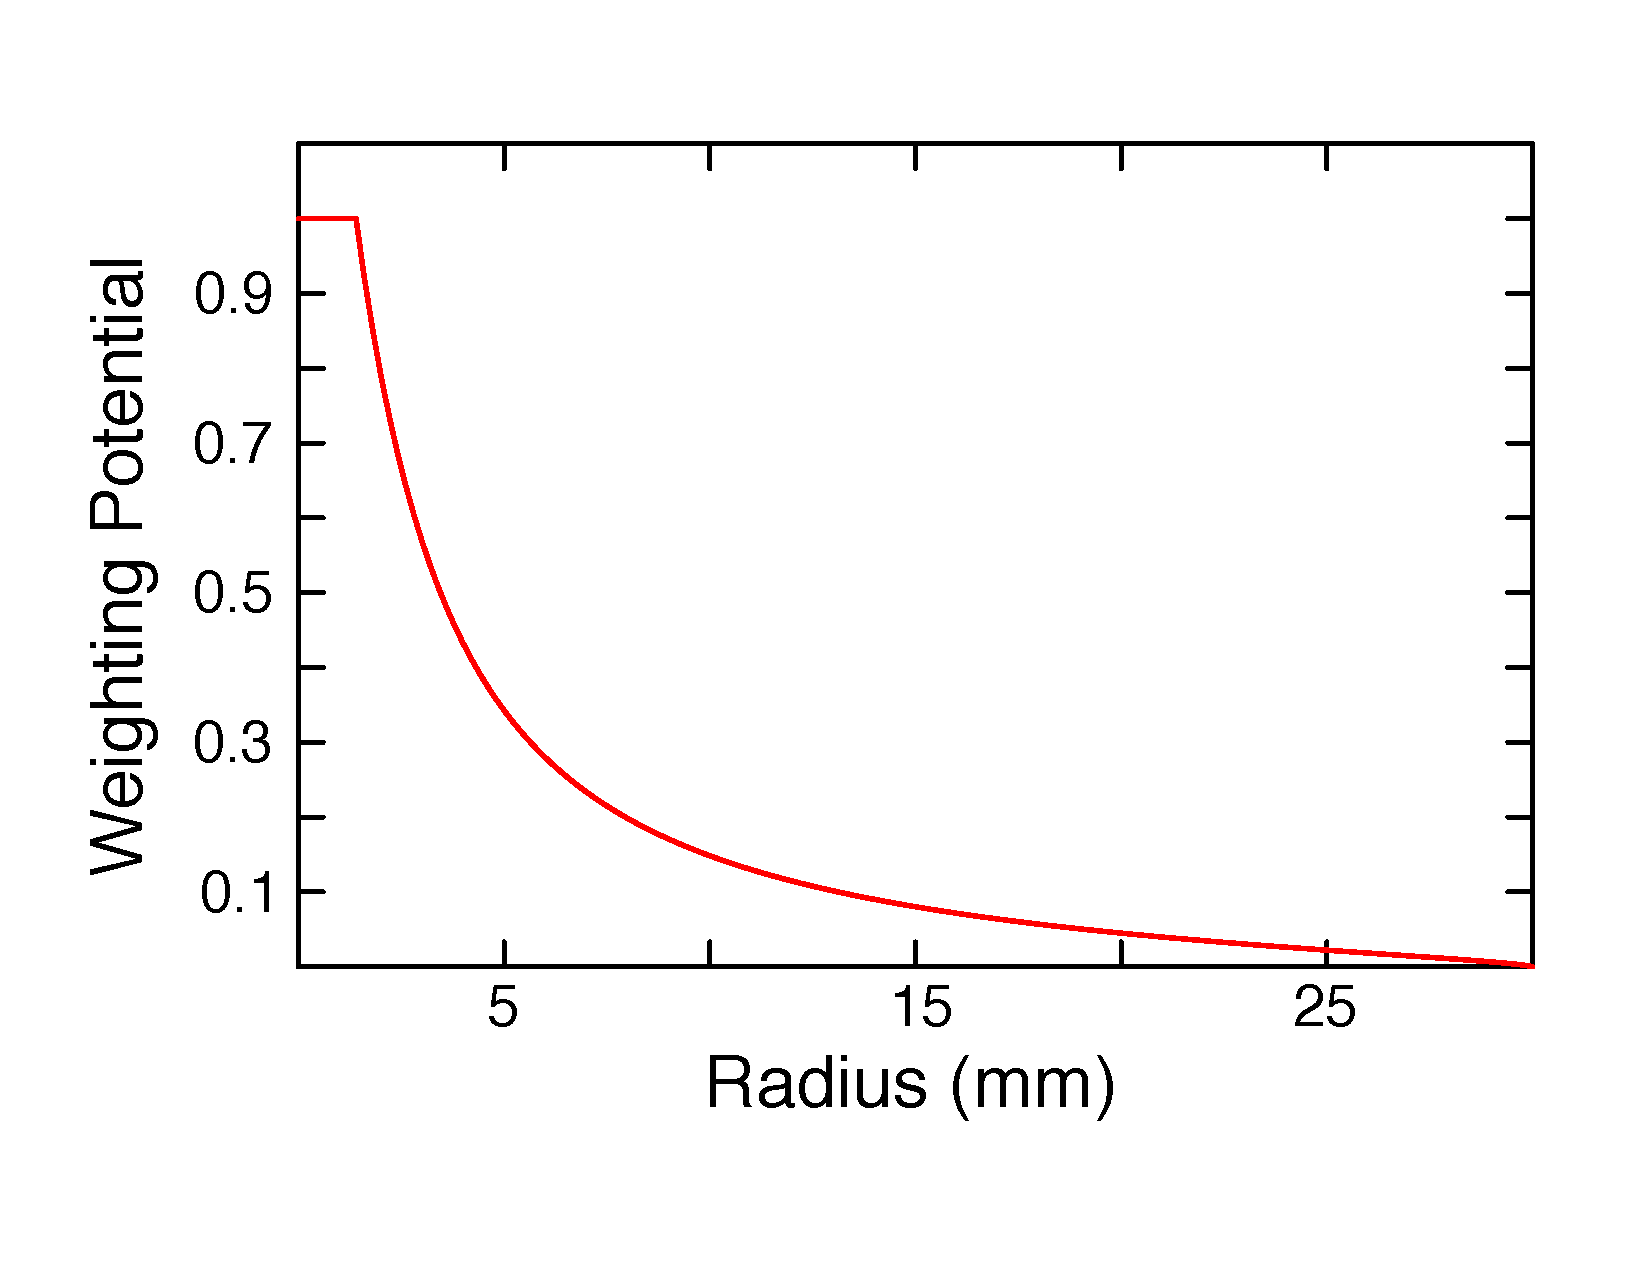
\includegraphics[height=3in]{/Users/jgruszko/Documents/Thesis/Plots/Ch6/wp_z0}
 \caption{The electron weighting potential at the passivated surface of a PPC detector similar to PONaMA-1. Calculated using {\tt fieldgen}.} 
 \label{fig:wp_z0}
\end{figure}

\section{DCR Parameter Values and Peak Shape}
\subsection{Observations}
In the DCR distribution for each data set, almost all alpha events fall in a gaussian peak. Fits to the alpha peaks in the DCR distributions are done for three of the parameters, {\tt dcr90}, {\tt dcrpzc90}, and {\tt dcrpzc99norm}. Deriving the results for alternate acceptance levels of the first two simply require a shift of the results, with no rescaling. The final version is provided to correct for the effects of gain shifts or changes in the pole-zero decay constant of the signal pulses, but is sensitive to changes in the noise of the system. 

\begin{figure*}[]
 \centering
  \begin{subfigure}[t]{.45\textwidth}
 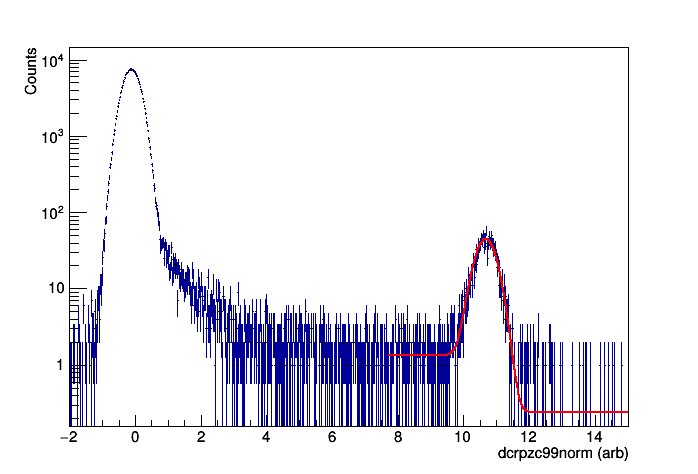
\includegraphics[width=1.0\columnwidth]{/Users/jgruszko/Documents/Thesis/Plots/Ch6/DS110_0_DCRPZCnorm.png}
  \caption{The {\tt dcrpzc99norm} distribution of a data set taken at 11 turns ($r= -13.5$\,mm), a total of 25.1\,hrs of runtime.}
 \label{fig:DCRfit_110}
\end{subfigure}
\hfill
  \begin{subfigure}[t]{.45\textwidth}
 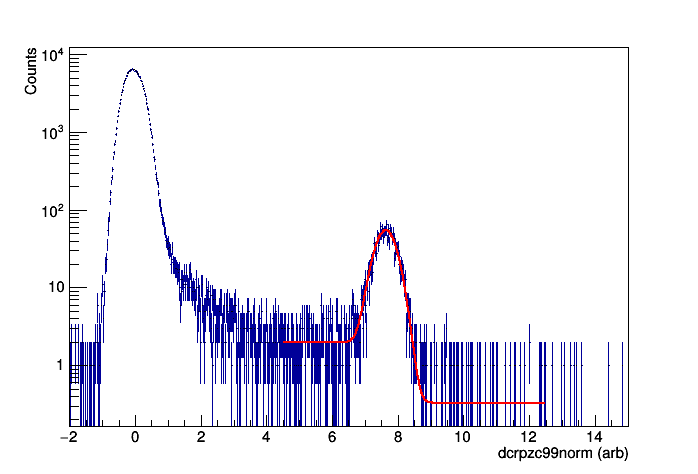
\includegraphics[width=1.0\columnwidth]{/Users/jgruszko/Documents/Thesis/Plots/Ch6/DS360_2_DCRPZCnorm.png}
  \caption{The {\tt dcrpzc99norm} distribution of a data set taken at 36 turns ($r = 24$\,mm), with 30.1\,hrs of runtime.}
 \label{fig:DCRfit_360}
\end{subfigure}
\hfill
 \begin{subfigure}[t]{.45\textwidth}
 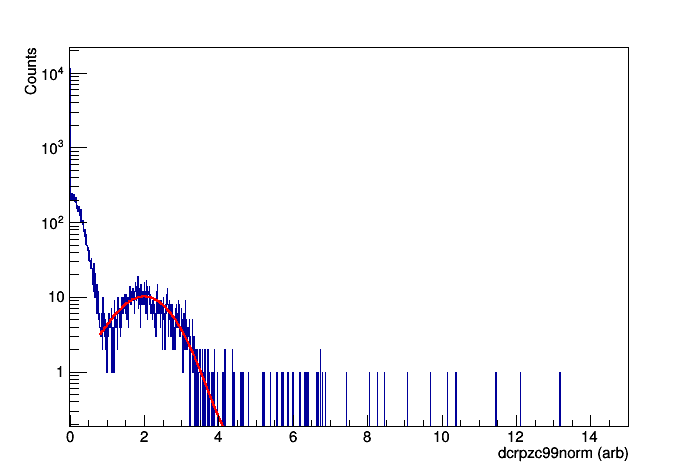
\includegraphics[width=1.0\columnwidth]{/Users/jgruszko/Documents/Thesis/Plots/Ch6/DS185_0_DCRPZCnorm.png}
  \caption{The {\tt dcrpzc99norm} distribution of a data set taken at 18.5 turns ($r = -2.25$\,mm), a total of 25.0\,hrs of runtime, with a cut selecting near-point-contact events (${\tt aenorm} > 1.5$). At small radii ($r<3$\,mm), the DCR parameter values for alpha events become similar to those of gamma background events.}
 \label{fig:DCRfit_185}
\end{subfigure}
\hfill
 \begin{subfigure}[t]{.45\textwidth}
 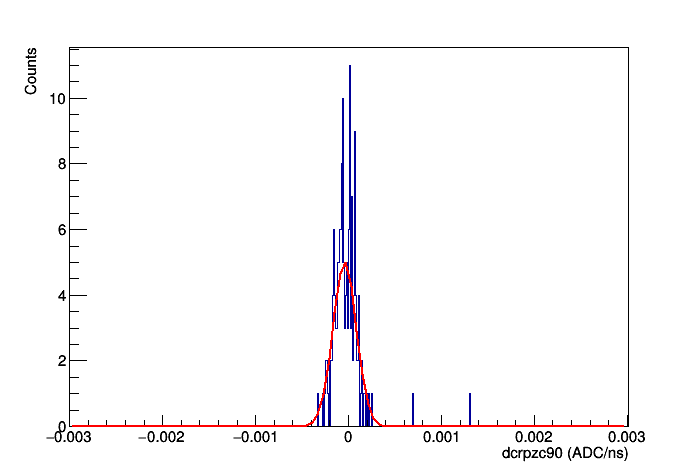
\includegraphics[width=1.0\columnwidth]{/Users/jgruszko/Documents/Thesis/Plots/Ch6/DS195_dcrpzcFit.png}
 \caption{The sum {\tt dcrpzc90} distribution of all runs taken at 19.5 turns ($ = -0.75$\,mm), a total of 82.4\,hrs of runtime, with a cut selecting near-point-contact events (${\tt aenorm} > 1.5$) in a $5\sigma$ energy window centered at the full-energy alpha peak position. Alphas incident on the point-contact do not show elevated DCR values.}
 \label{fig:DS195_dcrFit}
\end{subfigure}
 \caption[DCR parameter distributions and Gaussian fits for various peak positions]{DCR parameter distributions and Gaussian fits for various peak positions. The different varieties of DCR parameters generally have similarly-shaped distributions, save for peaks near 0 in {\tt dcrpzc99norm}, which are distorted by scaling effects. Fit results are given in Figs~\ref{fig:DCRfit} and \ref{fig:dcrNormFit}.} 
 \label{fig:DCRpeaks}
\end{figure*}

A full model-driven fitting function would include both a gaussian and exponentially-modified gaussian that accounts for the tail of low-DCR alpha events, seen in the plots of DCR vs. energy, in the fit to the peak. The background, which is the tail of the background-event gaussian, would be most appropriately modeled by a quadratic function. In practice, however, the fraction of alpha events occurring in the low-DCR tail small, and the relaxation constant of the tail is long. Combined with the low alpha rate, when a low-DCR tail is included, it is degenerate with the background function. Similarly, the inclusion of linear and quadratic components does not improve the fit to the background events. Instead, the combinations of the low-DCR tail of the signal and the low-DCR rise in the background can be fit effectively by including a step function (centered at the mean of the alpha peak gaussian) in the background function and limiting the fit window appropriately. Since the peak integral is not used for analysis, it is irrelevant whether the alpha peaks are fit with the signal or background components of the fit. 

The DCR spectrum includes all non-muon single-site events with energies between 1 and 6\,MeV. For $r > 3$\,mm, the energy of all observed alpha events falls in this range (see Table~\ref{tab:E_ranges}. Furthermore, the DCR value in the peak is sufficiently above the DCR distribution for normal events that the peaks can be clearly distinguished, and the high-DCR peak can be fit to a single Gaussian (see Figs~\ref{fig:DCRfit_110} and ~\ref{fig:DCRfit_360} for examples).

For data sets with $r<3\,mm$, the relevant energy range extends below 1\,MeV and the DCR values approach those of gamma background events, making the alpha event peak difficult to distinguish. As in the fits to the energy spectra, a pulse shape cut selecting near-point contact (${\tt aenorm} > 1.5$) events is applied to reduce the background rate and allow a fit to the alpha events (see Fig~\ref{fig:DCRfit_185}).

Events incident on the point contact itself do not have distinguishably distinct peaks in DCR when the broad energy range of 1 to 6\,MeV is used. Instead, the peak must be fit using an energy window in which the alpha events dominate the spectrum; a 5$\sigma$ window around the peak energy (taken from the fits described in Sec.~\ref{ssec:E_obs}) is used. Due to the low event and background rate after these cuts are applied, the peak is fit using only a Gaussian distribution. This approach is used only for the data sets with $r=-0.75$\,mm, the source position at which the beam is entirely incident on the point contact (see Fig~\ref{fig:DS195_dcrFit}).

All three of the DCR parameters are fit with the same procedure. The peak shapes in all three parameters are similar, save for at small radii ($r<6$\,mm), where the DCR parameter values are small and pole-zero corrected DCR parameters retain better alpha separation from the gamma and muon background events than the {\tt dcr90} value does. At very small DCR values, the {\tt dcrpzc99norm} peak shapes are distorted by the effects of the scaling on negative tail slope values. 

Results are given in Figs.~\ref{fig:DCRfit} and ~\ref{fig:dcrNormFit}. It is clear, both there and in the plots of the DCR values with respect to the magnitude of the radius (Figs.~\ref{fig:DCRfit_rMag} and ~\ref{fig:dcrNormFit_rMag}), that unlike the energy, the DCR parameter values of the alpha peaks do not appear to be azimuthally symmetric. At positions with $r>6$\,mm, the DCR values of alpha events are consistently much higher than those of background events; however, the value of the parameters differs by up to a factor of 2 at the $0\degree$ and $180\degree$ scanning positions. 

\begin{figure*}[]
 \centering
  \begin{subfigure}[t]{.45\textwidth}
 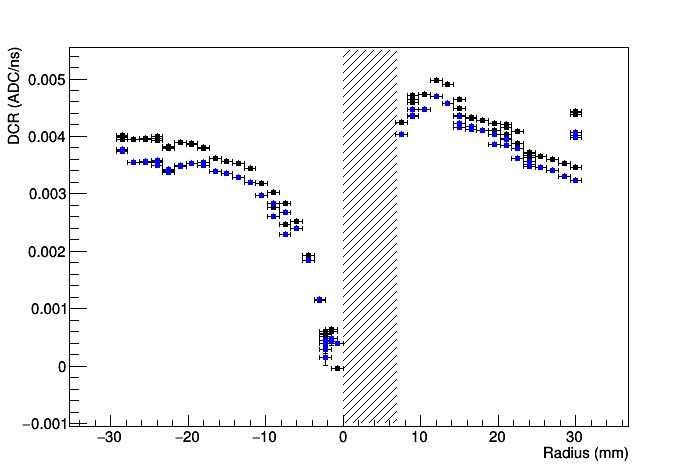
\includegraphics[width=1.0\columnwidth]{/Users/jgruszko/Documents/Thesis/Plots/Ch6/dcrCombined_mu.png}
 \caption{The centroids of the alpha peaks in each data set.} 
 \label{fig:DCRfit_mu}
\end{subfigure}
\hfill
\begin{subfigure}[t]{.45\textwidth}
 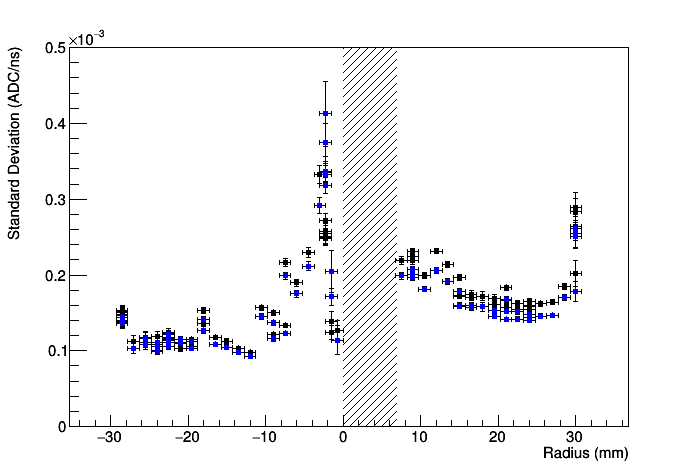
\includegraphics[width=1.0\columnwidth]{/Users/jgruszko/Documents/Thesis/Plots/Ch6/dcrCombined_sig.png}
 \caption{The standard deviation of the alpha peaks in each data set.} 
 \label{fig:DCRfit_sig}
 \end{subfigure}
 \caption[The results of Gaussian fits to the alpha peaks in {\tt dcrpzc90} and {\tt dcr90}]{The results of Gaussian fits to the alpha peaks in {\tt dcrpzc90}, in black, and {\tt dcr90}, in blue. All values are in units of ADC/ns. The hashed box indicates the region on the detector surface that is obscured by the contact pin and contact pin support.}
  \label{fig:DCRfit}
  
   \centering
  \begin{subfigure}[t]{.45\textwidth}
 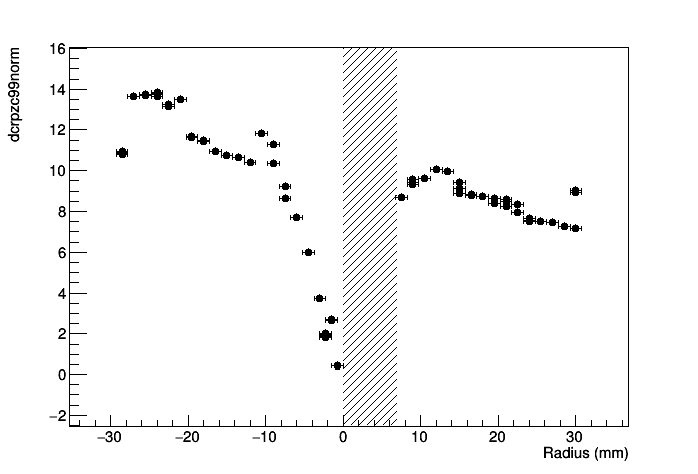
\includegraphics[width=1.0\columnwidth]{/Users/jgruszko/Documents/Thesis/Plots/Ch6/dcrpzc99normfit_mu.png}
 \caption{The centroids of the alpha peaks in each data set.} 
 \label{fig:dcrNormfit_mu}
\end{subfigure}
\hfill
\begin{subfigure}[t]{.45\textwidth}
 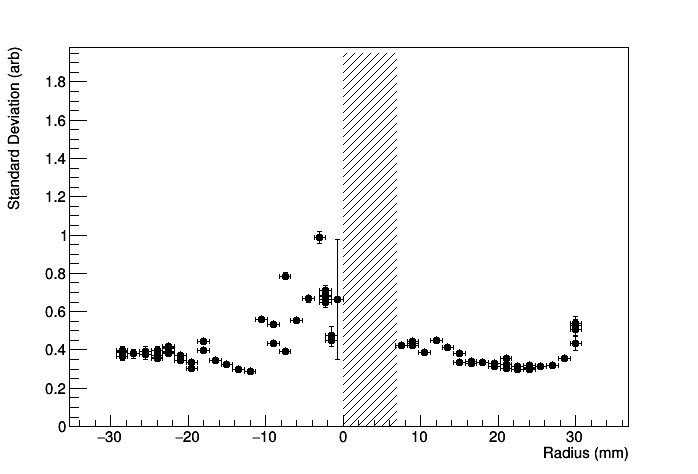
\includegraphics[width=1.0\columnwidth]{/Users/jgruszko/Documents/Thesis/Plots/Ch6/dcrpzc99normfit_sig.png}
 \caption{The standard deviation of the alpha peaks in each data set.} 
 \label{fig:dcrNormfit_sig}
 \end{subfigure}
  \caption[The results of Gaussian fits to the alpha peaks in {\tt dcrpzc99norm}]{The results of Gaussian fits to the alpha peaks in {\tt dcrpzc99norm}, in arbitrary units. The hashed box indicates the region on the detector surface that is obscured by the contact pin and contact pin support.}
  \label{fig:dcrNormFit}
\end{figure*}

Additionally, the positive and negative radius positions show different qualitative behavior for $r>12$\,mm. At the negative-radius positions, the DCR parameters values rise as the radius increases, and at positive-radius positions, their values fall with increasing radius. 

At positions with $r<= 12$\,mm, the $0\degree$ and $180\degree$ scans are in greater agreement, though their values of {\tt dcr90} and {\tt dcrpzc90} are still offset from one another, as in Fig.~\ref{fig:DCRfit_rMag}. Correcting for changes in the gain and noise of the system, as in \ref{fig:dcrNormFit_rMag}, brings the values at these radii into closer agreement. In this plot, it can also be seen that the DCR's functional dependence on radius is in agreement for these near-point contact positions. 

A discussion of the potential causes of the observed azimuthal dependence, along with further discussion of the DCR parameter significance, is given below. 

\begin{figure*}[]
 \centering
 \begin{subfigure}[]{\textwidth}
 \centering
 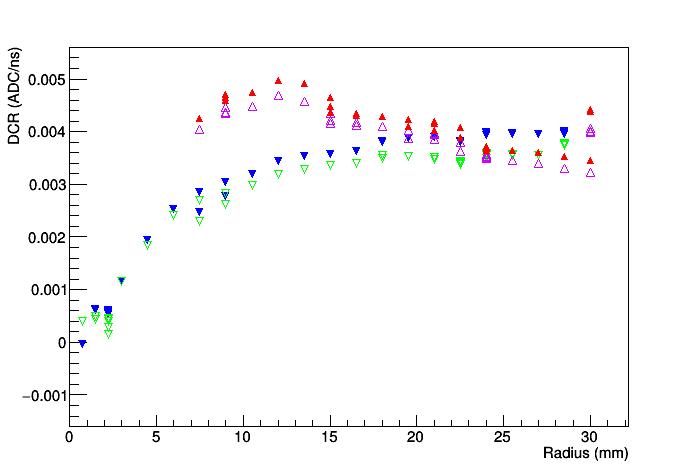
\includegraphics[height=3in]{/Users/jgruszko/Documents/Thesis/Plots/Ch6/dcrCombined_mu_rMag.png}
\end{subfigure}
 \begin{subfigure}[]{\textwidth}
  \centering
 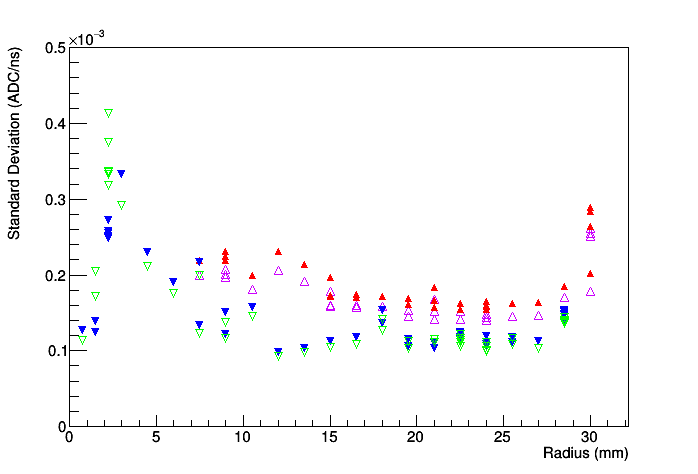
\includegraphics[height=3in]{/Users/jgruszko/Documents/Thesis/Plots/Ch6/dcrCombined_sig_rMag.png}
\end{subfigure}
 \caption[{\tt dcrpzc90} and {\tt dcr90} fit results as a function of distance from the point contact]{The centroids {\it (left)} and standard deviations {\it (right)} of the alpha DCR peaks in each data set, given as a function of the radial distract from the point contact. Both {\tt dcrpzc90} and {\tt dcr90} values are shown, in filled and open triangles, respectively. Error bars are suppressed for clarity. Negative-radius source positions appear as blue ({\tt dcrpzc90}) or green ({\tt dcr90}) downward-pointing triangles, and positive-radius positions as red ({\tt dcrpzc90}) or violet ({\tt dcr90}) upward-pointing triangles. The centroids of the 0$\degree$ and 180$\degree$ scans are not consistent with other another, but the peak widths appear relatively consistent. See~\ref{sssec:DCRfit_disc} for discussion.} 
 \label{fig:DCRfit_rMag}
\end{figure*}

\begin{figure*}[]
 \centering
 \begin{subfigure}[]{\textwidth}
 \centering
 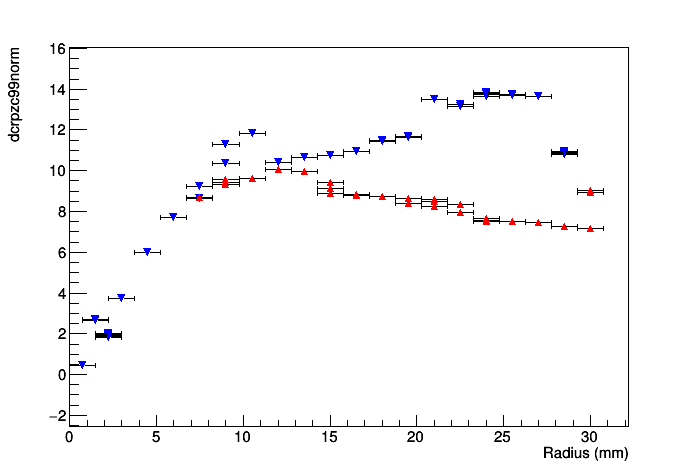
\includegraphics[height=3in]{/Users/jgruszko/Documents/Thesis/Plots/Ch6/dcrpzc99normfit_mu_rMag.png}
\end{subfigure}
 \begin{subfigure}[]{\textwidth}
  \centering
 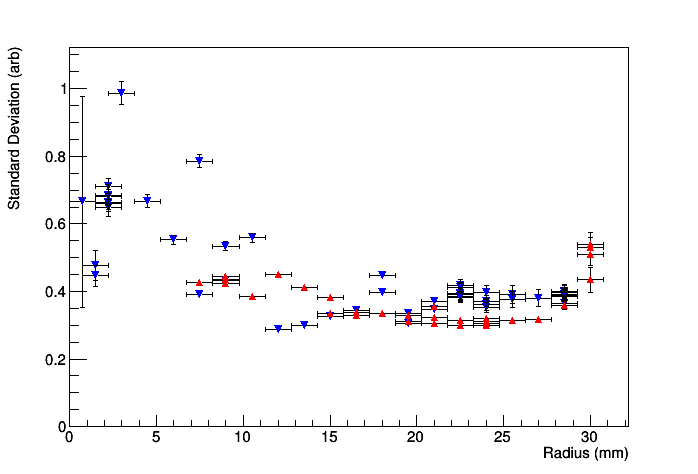
\includegraphics[height=3in]{/Users/jgruszko/Documents/Thesis/Plots/Ch6/dcrpzc99normfit_sig_rMag.png}
\end{subfigure}
 \caption[{\tt dcrpzc9norm} fit results as a function of distance from the point contact]{The centroids {\it (left)} and standard deviations {\it (right)} of the alpha {\tt dcrpzc99norm} peaks in each data set, given as a function of the radial distract from the point contact. The centroids of the 0$\degree$ and 180$\degree$ scans are not consistent with other another at $r>12$\,mm, but the peak widths appear relatively consistent. See~\ref{sssec:DCRfit_disc} for discussion.} 
 \label{fig:dcrNormFit_rMag}
\end{figure*}

\subsection{DCR as an Alpha Rejection Parameter}\label{sssec:DCRfit_disc}
At almost all scanning radii, alpha events incident on the passivated surface show significant slow charge components, and therefore highly elevated values of the DCR parameters. Therefore, the DCR pulse shape parameters provide a powerful tool by which external alpha events can be identified in PPC detectors. 

The amount of energy being collected as slow charge in the first 20\,$\mu$s of the pulse tail can be calculated directly from the {\tt dcrpzc90} parameter and the calibration constants for the electronics system. A {\tt dcrpzc90} value of 4E$-3$\,ADC/ns, similar to that found for many source positions, is divided by 0.74\,ADC/keV, the average value of the linear term of the energy calibration curve, to give an average rate of delated charge recovery in the pulse of 5.4\,keV/ns. The other terms of the calibration curve are relatively small, and are neglected. Therefore, in the 20\,$\mu$s of waveform tail that are digitized in these measurements, approximately 110\,keV of energy is collected. 

For each scanning position, we can find the slow component energy as a fraction of the prompt alpha peak energy at that position, as in Fig.~\ref{fig:Efrac}. The delayed charge energy fraction falls quickly at small scanning radii. At radii larger than 6\,mm, between 2.0 and 3.6\% of the total energy is collected as delayed charge, with an average delayed fraction of 2.5\%.  

\begin{figure}[]
 \centering
 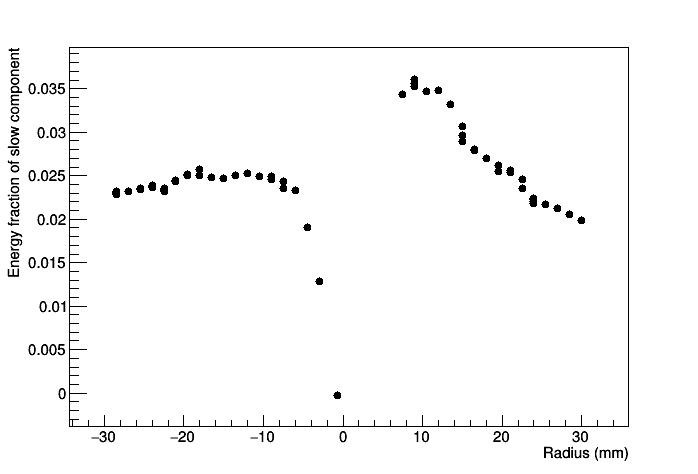
\includegraphics[height=3in]{/Users/jgruszko/Documents/Thesis/Plots/Ch6/slowFracOverE.png}
 \caption{The energy of the collected delayed charge, as a fraction of the prompt alpha energy at that scanning position.} 
 \label{fig:Efrac}
\end{figure}

The alpha background events of interest to rare event searches like the \MJ\ \DEM\ are those with energies of over 1\,MeV. Given the typical PPC detector energy resolution of less than 5\,keV at these energies, a 2\% delayed charge effect, corresponding to 20\,keV, is easily observable. This implies that regardless of the source of the alpha background, and whether the alpha particle is degraded in energy before reaching the passivated surface, any event that has high enough energy to be a problematic background event also demonstrates a detectable delayed charge signature, provided its point of incidence is at at a radius greater than 6\,mm. 

\subsection{Outlier Events}\label{sssec:outliers}
When we plot a given alpha scan data set in the DCR vs. energy parameter space, as in Fig.~\ref{fig:outliers}, some fraction of outlier events that do not fall either in the alpha energy or DCR peak also appear. This implies that the Gaussian model of the peak position and shape (in both energy and DCR) does not fully describe all of the observed alpha events. Some events have both degraded energies and DCR values. 

Significantly for our purposes, the fraction of the prompt energy that is collected as slow charge (i.e. the ratio of {\tt dcrpzc90}, in keV/ns and integrated over the duration of the waveform tail, to the energy) in these events appears to be constant, and is 2.9\%, identical to that of the undegraded events. This means that, as discussed in Sec.~\ref{sssec:DCRfit_disc}, these events can still be efficiently identified in the \nonubb\ ROI.

The fraction of events that appear as outliers in both parameters is impossible to calculate precisely, since they become indistinguishable from the statistical fluctuation of background events at low energies and DCR values. Based on the numbers of events at higher-than-usual DCR values, we estimate that approx. 10\% of events are outliers. 

It is difficult to speak to the physics of these outlier events, since we do not know their origin. The degraded outlier events could be caused by a dead layer or shallow angle scattering in the passivated surface itself. Therefore, events such as these could be useful in understanding further aspects of charge collection from surface events, and in measuring the dead-layer associated with the passivated surface. 

Though the source manufacturer cites a 20\,keV expected line-width for the $^{241}$Am source, that does not preclude the possibility of some small fraction of events being highly degraded in energy upon leaving the source. Another possibility is that these events are scattering in the collimator before arriving at the detector surface.

Alternatively, 

Given their consistent DCR energy fraction, it seems most likely that these 

Without knowing the origin of the outlier events, however, we cannot draw conclusions based on them. Future passivated-surface studies with the TUBE cryostat will employ source beams with shallower angles of incidence; based on the results of those studies, we should be able to determine the cause of these events and the thickness of the dead and charge-trapping regions associated with the passivated surface. 

\begin{figure}[]
 \centering
 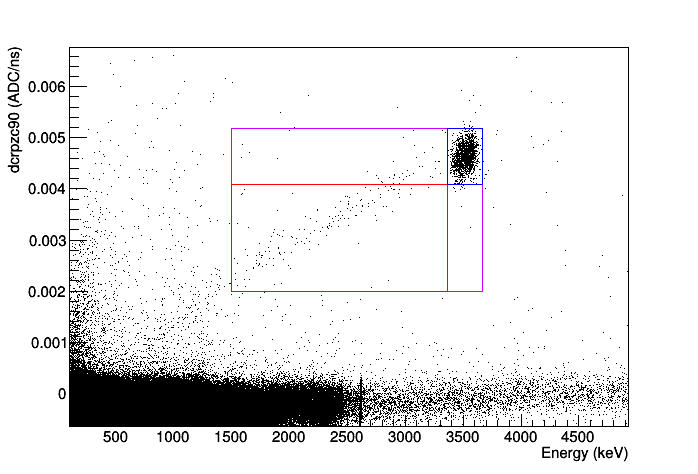
\includegraphics[width=1.0\columnwidth]{/Users/jgruszko/Documents/Thesis/Plots/Ch6/outlier_events_260_0.png}
 \caption[DCR vs. energy in a data set, showing outlier events]{A plot of all single-site events in a data set taken at $r=9$\,mm, in {\tt dcrpzc90} vs. energy. The blue box shows the region that lies within $5\sigma$ of the energy and DCR peaks, and the red box indicates some of the events that are outliers from both peaks. Events that are in the violet box but not in the red or blue boxes are outliers in either the energy or DCR peaks. The red-outlined region shows a clear excess of events over a source-free data set. 8.2\% of the events in the violet box (including the red and blue-boxed regions) are outliers from both peaks; 89.2\% fall within the $5\sigma$ windows of both the energy and DCR peaks.} 
 \label{fig:outliers}
\end{figure}


\subsection{Radial Dependence of DCR}
The azimuthal dependence (or, we believe, the instability, see below) of the DCR parameters makes it difficult to draw definitive conclusions about their radial dependence. This is particularly the case at large radii ($r>12$\,mm). In positive-radius scanning positions, {\tt dcrpzc90} falls with increasing radius, at a rate of -4.8E-5$\pm$1.2E-5\,ADC/ns/mm, found using a linear fit to all data sets in this position range. In negative-radius scanning positions, {\tt dcrpzc90} instead rises with increasing radius, at a rate of 2.8E-5$\pm$3E-6\,ADC/ns/mm. 

Compared to this, the radial dependence of the DCR parameters at positions with $r<12$\,mm is dramatic, and occurs with similar functional form in both the positive- and negative-radius scans, as seen in Figs. ~\ref{fig:DCRfit_rMag} and ~\ref{fig:dcrNormFit_rMag}. Unfortunately, the source beam is obstructed at small positive-radii positions, so the similarity of the results cannot be tested directly for all radii. 

Over the range that can be scanned, though, the positive-radius positions show a fall {\tt dcrpzc90} rise with increasing radius with a rate of 1.4E-4$\pm$3E-5\,ADC/ns/mm, and the negative-radius positions show an increase with the rate of 3.2E-4$\pm$2E-5\,ADC/ns/mm. If, instead of using all negative-radius data sets, we use only those for which a positive-radius equivalent exists, we derive a rate of change for the {\tt dcrpzc90} value of 1.8E-4$\pm$4E-5\,ADC/ns/mm, which agrees with the rate found at positive-radius positions to within the uncertainty of the fit. 

Most importantly, we find that at incidence positions very close to the point-contact ($r<6$\,mm), the DCR parameters cannot be used to reliably identify alpha events while retaining high bulk-event efficiency. Alphas incident on the point-contact itself are completely indistinguishable by their DCR parameters.   

\subsection{Stability of the DCR Value}
The apparent azimuthal dependence of the DCR value is thought, rather, to be a problem of instability in the process by which delayed charge is collected. 

The leading candidate for the cause of the shift in the DCR parameters is charging of the detector surface by the alpha particles themselves, and the resulting interactions in the detector surface. Passivated surface charge build-up over time has been observed in other PPC detectors (citation?), and our own measurements of the observed energy indicate that significant charge is being lost on or near the surface.
 
\begin{figure}[t]
 \centering
 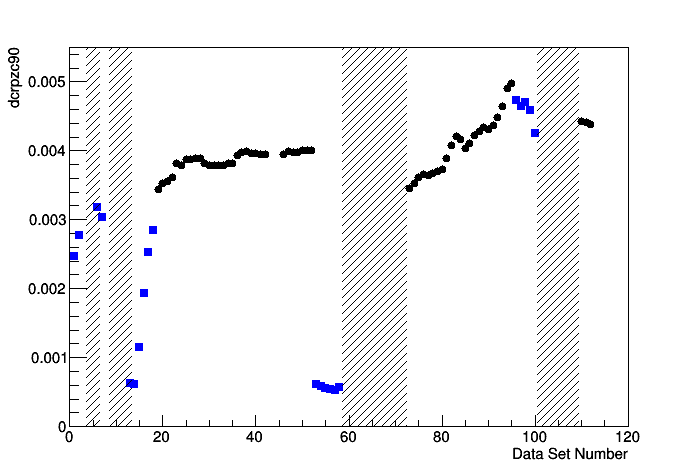
\includegraphics[height = 3in]{/Users/jgruszko/Documents/Thesis/Plots/Ch6/dcrpzc90fit_mu_overTime_allR.png}
 \caption[DCR scan results as a function of data set order, for all scanning positions]{The {\tt dcrpzc90} mean value of the alpha peak, as a function of data set order. One data set corresponds, almost exactly, to one day of run time. The hashed boxes indicates stretches of time during which the alpha source was not incident on the detector surface. The color scale indicates the alpha event rate, in events/hr. Results from scanning positions with $r>12$\,mm are shown as black circles, with results from those with $r<12$\,mm displayed as blue squares.} 
 \label{fig:DCRvT_all}
\end{figure}

In studies of the stability, data sets with $|r|<12$\,mm are excluded. Based on the observations of the radial dependence of DCR (above) and the DCR value over time (Fig.~\ref{fig:DCRvT_all}, it appears that at these positions, changes in the DCR value are dominated by the radial effects in the detector, and are unaffected by the azimuthal effect or instability, whatever its source. 

\begin{figure}[]
 \centering
 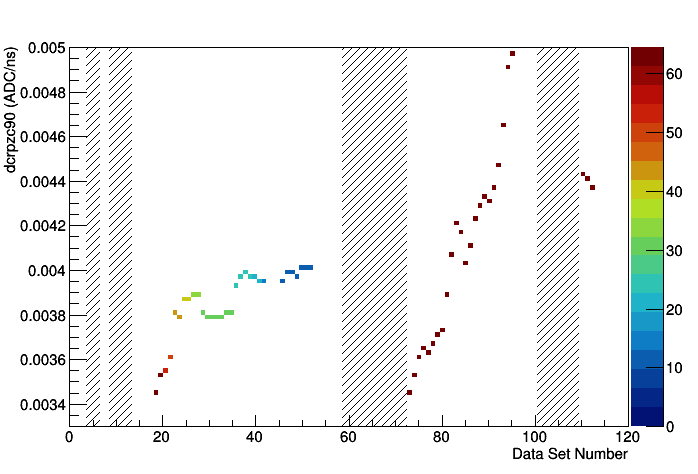
\includegraphics[width=1.0\columnwidth]{/Users/jgruszko/Documents/Thesis/Plots/Ch6/dcrpzc90fit_mu_overTime_rOver12_wRate.png}
 \caption[DCR scan results as a function of data set order, for |r|>12\,mm, including rate information]{The {\tt dcrpzc90} mean value of the alpha peak, as a function of data set order. One data set corresponds, almost exactly, to one day of run time. The hashed boxes indicates stretches of time during which the alpha source was not incident on the detector surface. The color scale indicates the alpha event rate, in events/hr.} 
 \label{fig:DCRvT}
\end{figure}

Plotting {\tt dcrpzc90} in each data set with respect to the data set order (which corresponds, almost exactly, to days of run time), as in Fig.~\ref{fig:DCRvT}, shows a pattern in which the DCR parameter values rise over the time during which the source is incident on the passivated surface, ``resetting" to lower values after the source beam is removed from the surface for some time. Furthermore, the rate at which the DCR value increases appears to be correlated with the observed alpha rate, as would be expected if surface charge build-up were the cause of the change. 

Additional evidence for this theory is provided by the changes in DCR values in the positions that were repeated non-consecutively, with several days of scanning of other positions occurring between the two scans at that location. This was done for 5 positions, at $r= $ -15, -9, -7.5, -4.5, and 30\,mm. In all three cases, shown in Fig.~\ref{fig:DCR_repeated}, the second measurement shows a higher DCR value than the first measurement.  

\begin{figure}[t]
 \centering
 \begin{subfigure}[]{.7\textwidth}
 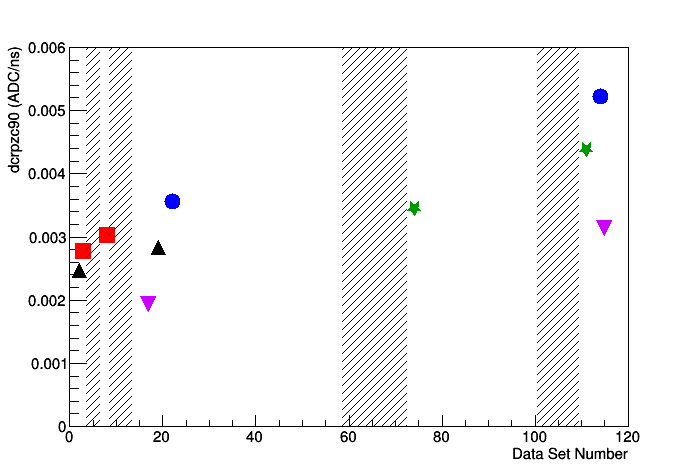
\includegraphics[height=3in]{/Users/jgruszko/Documents/Thesis/Plots/Ch6/dcrpzc90fit_mu_overTime_repeatedPos.png}
 \end{subfigure}
  \begin{subfigure}[]{.25\textwidth}
 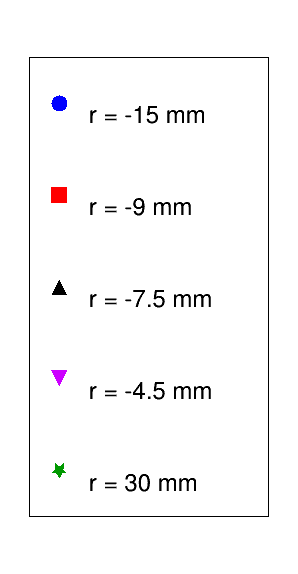
\includegraphics[height = 3in]{/Users/jgruszko/Documents/Thesis/Plots/Ch6/dcrpzc90fit_mu_overTime_repeatedPos_leg.png}
  \end{subfigure}
 \caption[The change in DCR parameter values over time at repeated scan positions] {The {\tt dcrpzc90} mean value of the alpha peak as a function of data set order for the non-consecutively repeated measurements. The point shape and color indicate the position of the source, as given by the legend. The hashed boxes indicates stretches of time during which the alpha source was not incident on the detector surface.} 
 \label{fig:DCR_repeated}
\end{figure}

In spite of the observed instability, the DCR value at smallest re-measured radius ($r =-4.5$\,mm) remains smaller than those of the larger-radius positions scanned soon before and after it. This is a good indication that there is radial variation in DCR along with the variation over time.


\section{A/E and DCR: Complementary Pulse-Shape Discriminators} 
\subsection{A/E of Surface Alpha Events}
As expected from the calculated drift paths of PPC detectors, the rate of the initial rise of pulses strongly depends on the event incidence radius, particularly near the passivated surface. The high-A/E peak of events associated with the alpha source was fit using a Gaussian function, and its centroid $\mu_{AE}$ was taken as the characteristic A/E value of the scanning location. Since the precise peak shapes of the A/E distributions are not of interest for this work, we use a simplified fitting model, with only a Gaussian component to identify the peak centroid and width. 

For runs in which the energy of the $\alpha$ peak is well over 2630\,keV ($\abs{r} > 7.5$\,mm), only events with energies between 2630\,keV and 6\,MeV are included. For data sets with $\abs{r} < 7.5$\,mm, where all or some of the alpha peak may fall outside this energy window, events with energies between 1 and 6\,MeV are included. See Fig.~\ref{fig:AE_fits} for sample A/E distributions and fits. 

\begin{figure*}[]
 \centering
 \begin{subfigure}[t]{.45\textwidth}
 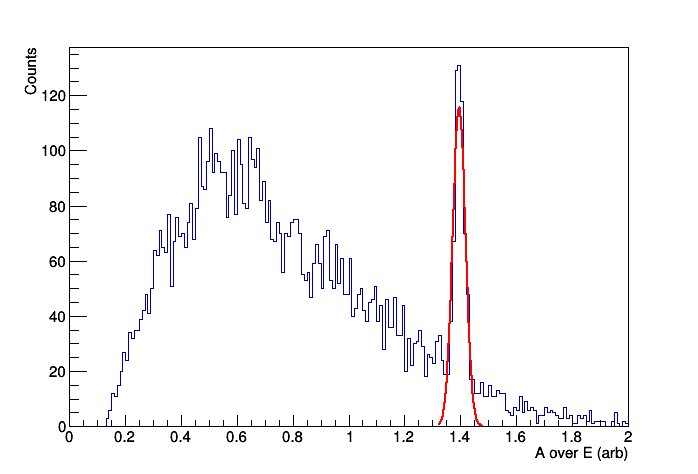
\includegraphics[width=1.0\columnwidth]{/Users/jgruszko/Documents/Thesis/Plots/Ch6/DS10_0_aefit.png}
 \caption{A data set taken at 1 turn ($r=-28.5$\,mm), a total of 24.9\,hrs of runtime, with a cut selecting events with energy between 2630\,keV and 6\,MeV.}
\end{subfigure}
\hfill
 \begin{subfigure}[t]{.45\textwidth}
 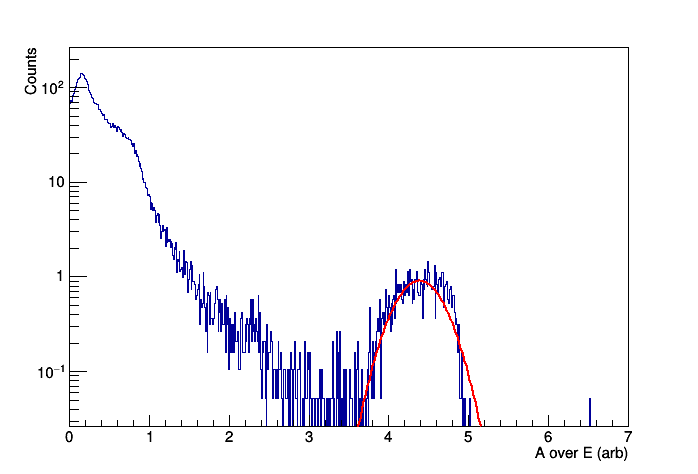
\includegraphics[width=1.0\columnwidth]{/Users/jgruszko/Documents/Thesis/Plots/Ch6/DS170_0_aefit.png}
  \caption{A data set taken at 17 turns ($r=-4.5$\,mm), a total of 19.1\,hrs of runtime, with a cut selecting events with energy between 1\,MeV and 6\,MeV.} 
\end{subfigure}
\caption[Sample A/E distributions and Gaussian peak fits to alpha events]{Sample A/E distributions and Gaussian peak fits to alpha events.}
 \label{fig:AE_fits}
\end{figure*}

For most data sets, the peak in A/E is approximately Gaussian in shape. As in the case of energy, the peak becomes non-Gaussian at small radii, where the length scale of significant changes to the drift time of charges becomes small compared to the diameter of the source beam. At these small radii, however, the A/E values are well above those of 99\% of background events. 

Anomalously low values of A/E occur for events incident on the point-contact itself. Though these events have very fast rising edges, they also have a substantial slow electron fraction, which reduces the A/E value. To correctly identify events like these from the shape of their rising edge, a rise-time parameter, measuring time over which the pulse rises from the start of the prompt signal to a given fraction of its total amplitude (for instance, 50\% of the maximum pulse height), would be more appropriate than the A/E parameter used in this analysis. The \MJ\ Collaboration plans to implement such a pulse-shape discriminator, in addition to the {\tt avse} parameter that is currently used to reject multi-site events.

\begin{figure}[t]
 \centering
 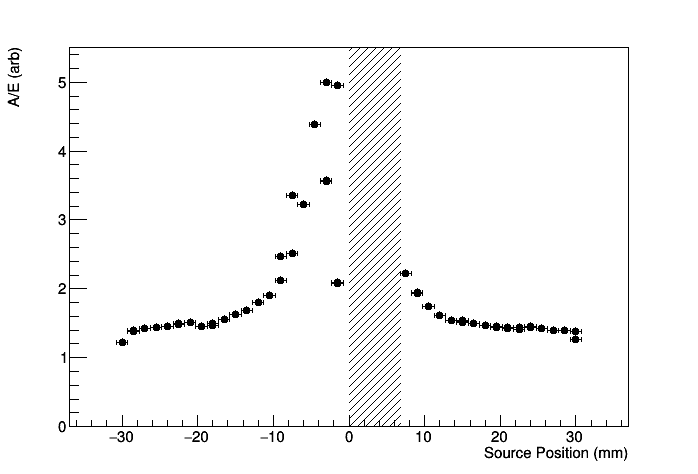
\includegraphics[height=3in]{/Users/jgruszko/Documents/Thesis/Plots/Ch6/AEvR_wBox.png}
 \caption[The results of fits to A/E in each data set]{The centroids of the alpha peaks in A/E in each data set. The relatively low value of A/E for data sets with $r=-0.75$\,mm occurs because the large (relatively slow) electron component of the signal reduces the A/E value for these events.} 
 \label{fig:AEfit_mu}
\end{figure}

The fit results are displayed in Fig.~\ref{fig:AEfit_mu}. These results indicate that the high-A/E cut applied to give energy and DCR fit results,  as in Sec.~\ref{ssec:E_obs}, is appropriate.


\subsection{Demonstrating Complementarity of High-A/E and DCR Cuts}
The distributions of alpha events incident at various radii in the A/E vs. DCR parameter space (see Fig.~\ref{fig:AEvDCR_events}) suggest that the two pulse-shape analyses are highly complementary. This suggests that by using both the A/E and DCR pulse shape discriminators, we should be able to achieve excellent alpha event discrimination with only minimal sacrifice of bulk events. 

\begin{figure*}[]
 \centering
 \begin{subfigure}{.65\textwidth}
 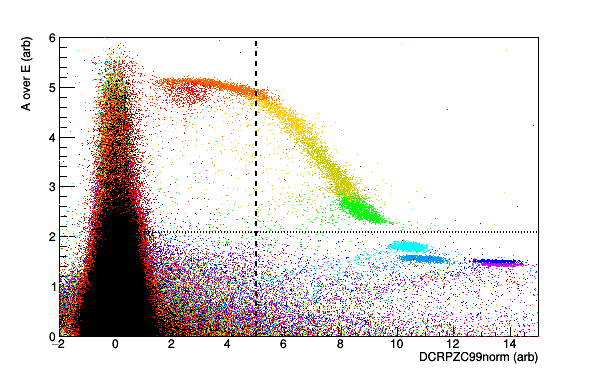
\includegraphics[width=1.\columnwidth]{/Users/jgruszko/Documents/Thesis/Plots/Ch6/AEvDCRPZCnorm.png}
 \end{subfigure}
 \begin{subfigure}{.34\textwidth}
  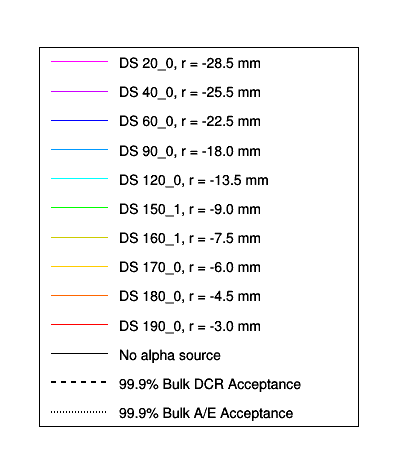
\includegraphics[width=1.\columnwidth]{/Users/jgruszko/Documents/Thesis/Plots/Ch6/AEvDCR_plot_legend.png}
   \end{subfigure}
 \caption[The A/E vs. normalized DCR distribution at various scanning radii]{The A/E vs. normalized DCR distribution for all single-site events with energies between 100\,keV and 10\,MeV, at various scanning radii. The points in black are from a data set without the alpha source incident on the detector surface, and the scan data sets are shown in rainbow order, with red representing the smallest-radius scan. 99\% of calibration events with energies between 1000 and 2630\,keV fall below an A/E value of 1, and 99\% of calibration events with energies between 1000 and 2380\,keV fall below a {\tt dcrpzc99norm} value of 1.} 
 \label{fig:AEvDCR_events}
\end{figure*}

Examining the fit results to the DCR and A/E peaks supports this conclusion. The $5\sigma$ windows around each alpha peak should include 99\% of the events, assuming normally distributed values; by using an equivalent normalization for the A/E and DCR values, we can compare them directly, as in Fig.~\ref{fig:AEandDCR}. The y-axis in this figure indicates the alpha events' separation from bulk events-- 99\% of bulk events fall below 1, whether the relevant discrimination parameter is A/E or DCR. Also indicated are the 99.9\% acceptance points in each parameter, which occur at different values for A/E and DCR, indicating that the DCR distribution is more heavily-tailed than the A/E distribution. 

\begin{figure*}[]
 \centering
 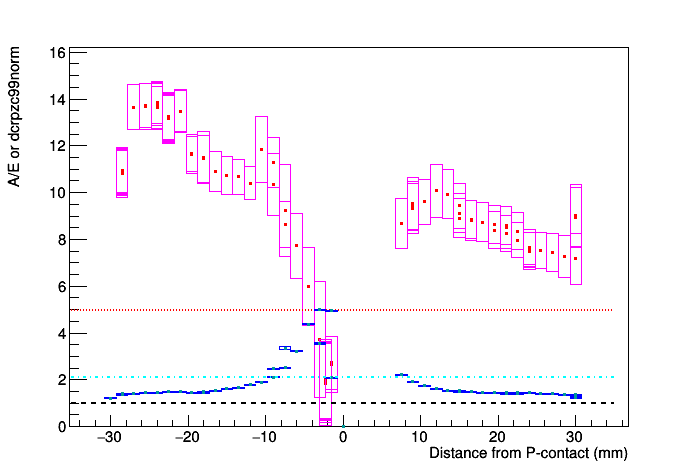
\includegraphics[width=1.\textwidth]{/Users/jgruszko/Documents/Thesis/Plots/Ch6/AEandDCR_noThree.png}
 \caption[A plot of A/E and DCR alpha peak positions, showing the complementarity of the pulse shape discriminators]{The $5\sigma$ window containing the A/E and DCR alpha peak positions at each position, normalized to 99\% bulk acceptance of both cuts. The red points and magenta boxes indicate the centroids and $\pm 2.5\sigma$ values of the peaks in {\tt dcrpzc99norm}, and the green points and blue boxes indicate the same in {\tt aenorm}. The red dotted line and cyan dotted-dashed line are the 99.9\% acceptance points in DCR and A/E, respectively. The black dashed line indicates the 99\% acceptance point in both parameters.} 
 \label{fig:AEandDCR}
\end{figure*}

For each position measured, we find that either or both of the DCR and A/E discriminator parameters are well above the 99.9\% acceptance line for that parameter. This indicates that by applying 99.9\% bulk-acceptance cuts in both parameters, we can effectively eliminate alpha events occurring anywhere on the passivated surface. Ergo, total alpha event rejection with only 0.2\% sacrifice of bulk events should be possible in PPC detectors.

Another advantage of this method of alpha removal is that it is equally effective at all energies of the alpha events, save for the requirement that the energy of the event be high enough that the DCR signal (of approximately 2-3\% of the prompt event energy, see above) is detectable. This is the case for all events that could fall in the \nonubb\ ROI. Therefore, this purely pulse-shape-based method is as effective for energy-degraded alpha events as it is for undegraded events originating from alpha contamination on the surface itself.

The only exception to this highly efficient alpha event removal occurs for events directly incident on the point-contact itself, at the smallest-radius position. Given that these events do not experience charge trapping, their energies are much higher than that of the \nonubb\ region-of-interest, so they are not a particularly problematic background. If alpha energy is degraded before reaching the point-contact, though, they could have any energy below the full energy of the alpha peak. As discussed above, these events would be effectively tagged with high efficiency if a rise-time parameter were substituted for the A/E parameter, as is planned in the \MJ\ \DEM\ analysis. 

Fig.~\ref{fig:AEandDCR} also shows that at positions with $r<= 6$\,mm, the A/E-based rejection of alpha events dominates in effectiveness, and that below $r=9$\,mm, an 99.9\%-acceptance cut in A/E suffices to tag all alpha events. This is why the previous study of alpha backgrounds in a PPC detector \cite{Agostini_thesis}, found no need for an additional pulse-shape discriminator beyond A/E, though an asymmetry parameter, which identifies slowly-released charge like our DCR parameter, was studied \cite{TUBEdoc?}. BEGe-type detectors, like the one measured in that work, have the entirety of their passivated surface lying within $r=9$\,mm, so the use of the DCR discriminator would not measurably improve their background rejection capabilities. 

The DCR discriminator is needed, though, in ORTEC-type detectors, which have a passivated surface along the entire bottom plane of the detector. In this detector design, which is that of the detector measured in this work, and used for all of the \MJ\ \DEM 's enriched detectors, the DCR discriminator is a powerful way to reject alpha events occurring far from the point-contact, where A/E is relatively insensitive. 

\subsection{Alpha-Identification Efficiency using DCR Techniques}
Given that the DCR pulse-shape discrimination technique is less effective than the A/E technique at $r<=6$\,mm, we focus our attention on evaluating the alpha-rejection efficiency of the various DCR parameters at scanning positions with $r>6$\,mm. 

To calculate an alpha-rejection fraction, we must first find the predicated number of background events in the alpha peak region of the data set, with no DCR cut applied. We use both the right-hand sideband in the data set and the spectral shape in the sideband and peak regions, measured in a source-free run, to find the expected number of background events. See Fig.~\ref{fig:eff_regions} for sample spectra and energy regions. 

\begin{figure*}[]
 \centering
 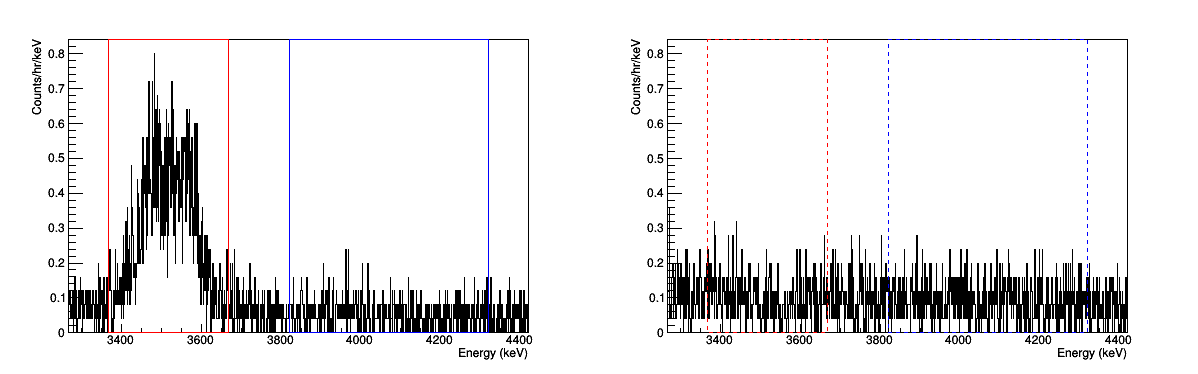
\includegraphics[width=1.\textwidth]{/Users/jgruszko/Documents/Thesis/Plots/Ch6/eff_peakRegions.png}
 \caption[Energy spectra, showing the windows used to calculate the DCR alpha rejection efficiency]{Energy spectra for a source scan data set with $r=9$\,mm {\it (left)} and a background data set {\it (right)}. The energy windows indicated are the $5\sigma$ peak region, in red, and the 500\,keV right-hand sideband, in blue. $n_{s, pk}$ is the sum of all events in the red solid-lined box and $n_{s, rh}$ is the sum of all the events in the blue solid-lined box. $n_{b, pk}$ and $n_{b, rh}$ are the sum of events in the red and blue dashed-line boxes, respectively.} 
 \label{fig:eff_regions}
\end{figure*}

Below, the background data set is referred to by the subscript {\it b} and the alpha source scanning data set by the subscript {\it s}. The peak region is taken to be a $5\sigma_E$ window around the centroid of the alpha-energy Gaussian, and the sideband region is the 500\,keV region with minimum energy of $\mu_E+5\sigma_E$. Only a right-hand sideband is used, to avoid effects from the energy-degraded alpha events described in Sec.~\ref{sssec:outliers}. The peak region is referred to by the subscript {\it pk}, and the sideband region by the subscript {\it rh}.

The following algorithm is repeated for each alpha scan data set for which we would like to calculate the efficiency:
\begin{itemize}
\item The expected spectral shape of the background events is calculated from a background run. To do this, the number of events in the peak region, $n_{b, pk}$, and the number of events in the right-hand sideband region, $n_{b, rh}$ are found. Each event total is divided by the width of its energy window. Their ratio is the number of events per keV expected in the peak region, given some number of events per keV in the sideband region.
\item The number of events in the right-hand sideband of the source scan data set, $n_{s, rh}$ is found. It is normalized by the width of the sideband energy window, and then multiplied by the width of the peak energy window and the spectral shape ratio to give the number of background events per hour expected in the peak region. 
\item This value is subtracted from the measured number of peak-region events in the alpha source scan data set, $n_{s, pk}$ to give the projected number of alpha events, $n_{\alpha}$. I.e., 
$$ n_{\alpha} =  n_{s, pk}-n_{s, rh}\frac{n_{b, pk}}{n_{b, rh}}\frac{5\sigma_E}{500\,keV} $$
\item The above steps are repeated after the DCR cut is applied to both the source and background runs to find the expected number of background events in the peak region of the source scan data set that would be removed by the cut. This value is subtracted from the total number of events cut in the peak region of the source data set to give the projected number of alpha events removed by the cut, $m_\alpha$. I.e.,
 $$ m_{\alpha} =  m_{s, pk}-m_{s, rh}\frac{m_{b, pk}}{m_{b, rh}}\frac{5\sigma_E}{500\,keV} $$
 where the $m_{i, j}$ are equivalent to the $n_{i, j}$ above, but measured after the DCR cut is applied. 
\item The ratio $\frac{m_\alpha}{n_\alpha}$ is the alpha rejection efficiency in the source-scan data set. 
\end{itemize}

A derivation of the formula by which the uncertainties for these efficiencies are calculated is given in Appendix FIXME. 

At positions with radii below 6\,mm for which the source is incident on the passivated surface, the alpha peak appears in a region of the energy spectrum that is dominated by gamma background events from environmental radioactivity and the materials of the cryostat itself. The alpha event rate is low, and these backgrounds are both high and highly variable. An additional complication comes from the broad energy distribution of the alpha events at these positions, as discussed in Sec.~\ref{ssec:E_obs}; to find an expected alpha event rate, we must understand the spectral shape over the entire range of relevant energies with high accuracy. 

This implies that our approach of normalizing the background spectra to one another is of limited utility.  The resulting uncertainties from the estimate of the backgrounds dominate our expected alpha event rate. Without an accurate calculation of the expected number of alpha events, we cannot accurately cite a rejection fraction for the events. Therefore, measurements at these radii are not included in the average efficiency values for each DCR parameter. 

Events incident on the point-contact itself are not expected to exhibit slow charge release, and are therefore expected to be relatively unaffected by the DCR cut. Data sets with the source beam incident on the point-contact are therefore also excluded from the average efficiency calculations. 

The rejection efficiencies are calculated for each data set using the {\tt dcr90}, {\tt mjddcr90}, and {\tt dcrpzc90}, and {\tt dcrpzc99norm} parameters. The first three of these are set to retain 90\% of single-site calibration events, and the final cut is set to retain 99\% of calibration events. The results for each data set are shown in Fig.~\ref{fig:eff_allR}, and the average rejection efficiency values for each parameter are given in Table~\ref{tab:avgEff}. 

The errors for the efficiency of each data set are large, due to the low alpha rate. They are particularly large at positions with large-magnitude negative radii, where the source beam is partially obscured. 

Averaging the efficiency at all scanning positions, however, reduces the error sufficiently to show that the rejection efficiencies of the various DCR parameters, save for {\tt dcrpzc99norm}, are consistent with 99\%. This implies that 1\% of alpha events with the full expected energy (indicating that significant charge trapping has occurred) are not measurably re-releasing that charge on the time scale of digitization. The higher average efficiency of the normalized DCR parameter ({\tt dcrpzc99norm}), which is consistent with 100\%, suggests that the culprit may be varying noise in the system, which is corrected for by the use of this parameter. This is unsurprising, given the high noise (and particularly the high and varying levels of microphonic noise, due to the vacuum pump operation) in the TUBE scanning setup. 

\begin{figure*}[]
 \centering
 \begin{subfigure}[]{\textwidth}
 \centering
 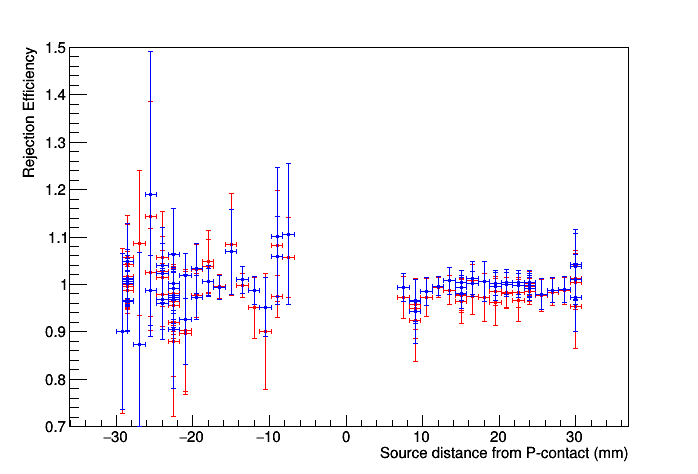
\includegraphics[height=3in]{/Users/jgruszko/Documents/Thesis/Plots/Ch6/dcrpzc_eff.png}
 \caption{The DCR parameters that employ event-by-event pole-zero correction. Values for {\tt dcrpzc90} are in red, and those for {\tt dcrpzc99norm} are in blue.} 
 \end{subfigure}
 \hfill
  \begin{subfigure}[]{\textwidth}
  \centering
 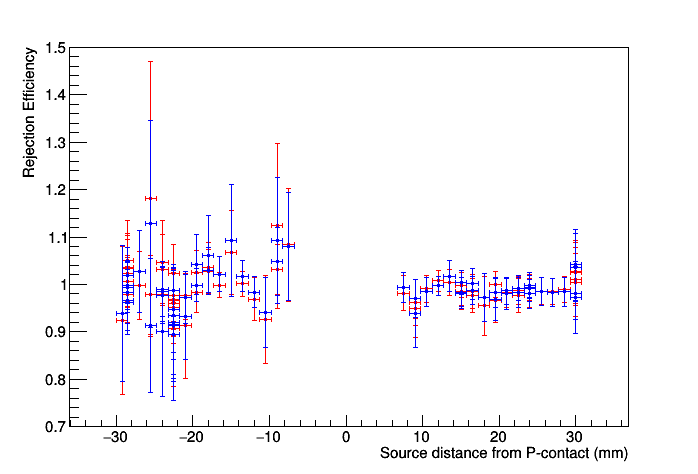
\includegraphics[height=3in]{/Users/jgruszko/Documents/Thesis/Plots/Ch6/dcr_eff.png}
 \caption{The DCR parameters that employ the linear projection method of pole-zero correction. Values for {\tt dcr90} are in red, and those for {\tt mjddcr90} are in blue.} 
 \end{subfigure}
 \caption[The alpha rejection efficiency as a function of radius for each DCR parameter]{The alpha rejection efficiency of each DCR parameter, calculated for each data set with a source beam incidence position with $r>6$\,mm.}
 \label{fig:eff_allR}
\end{figure*}

\begin{table}[]
\begin{center}
\begin{tabular}{l r r}
DCR Param. & ~~$\varepsilon$ (\%), $|r|>6$\,mm \\  \hline
{\tt dcr90} & 99.2$\pm$0.5  \\
{\tt dcrpzc90} & 98.9$\pm$0.5  \\
{\tt mjddcr90} & 99.1$\pm$0.5  \\
{\tt dcrpzc99norm} &  99.7$\pm$0.4 \\
\end{tabular}
\caption{Average alpha rejection efficiencies for all evaluated DCR parameters.} \label{tab:avgEff}
\end{center}
\end{table}

\section{Comparison to Models of Surface-Charge Collection}\label{sec:dcr_models}
\subsection{Surface Drift of Electrons}
The original theoretical model for the DCR effect posited that slow surface-drift of electrons was responsible for the slow charge component, with holes being collected normally through the bulk \cite{Neutrino16}. Charge transport models in germanium \cite{Mullowney2012} suggest that charge carrier mobilities are 10 to 100 times slower for surface transport than for bulk transport. Given the overall lower mobility of electrons, and the lower weighting potential they experience over much of the detector surface (as in Fig.~\ref{fig:wp_z0}), we would expect that electrons would be much more susceptible to surface transport than electron holes. 

This effect can be modeled using the {\tt fieldgen} and {\tt siggen} software packages by generating the fields in the detector with the addition of a small amount of charge deposited on the passivated surface. This creates drift paths that run perpendicular to the passivated surface in a narrow region near the surface. Events that occur in this skin depth, like alpha interactions, will have degraded energies and a DCR contribution (see Fig.~\ref{DCR_wf}). Electrons that reach the surface as assigned a slower drift speed, in this case a factor of 2\% of the bulk drift speed (check this with Susanne). 

The radial dependence of energy, in this case, mimics the inverse of the electron weighting potential exactly, since the fraction of the signal carried by the electrons is missing at all radii (see Fig.~\ref{fig:sim_EvR_e}). Because the electron component of the pulse shape (which is the origin of the DCR signal, in this case) increases in strength at small radii, we would expect that the DCR effect would  be particularly large at radii very near to the point-contact radius. In general, it would be expected to decrease with increasing radius, as in Fig.~\ref{fig:sim_DCRvR_e}. 

Given the observed radial dependence of energy and DCR, this model is not confirmed by the TUBE measurements. Though surface drift of electrons may be occurring, it is not the dominant effect observed. 

\subsection{Passivated-Surface Trapping of Holes}
An alternative model, in which the collection of the electron-holes is also impeded by the passivated surface layer effects, was developed. If there is a high concentration of bulk trapping centers in a thin layer near the passivated surface, as suggested by the direct measurements of trapping made in segmented germanium detectors ~\cite{Abt2017}, then some fraction of the electron-holes will be trapped in the bulk of the detector. Slow rerelease of these charges would lead to a DCR effect, in addition to the prompt signal from untrapped electron-holes. The rate of this rerelease would be temperature-dependent \cite{?}. Additionally, the electron fraction is completely or almost completely lost to trapping or slow surface transport in this model, which as in the surface-electron model, is likely given electrons' lower mobility. 

Again, we model the resulting radial dependence of energy and the DCR parameter using {\tt siggen}. The electron contribution to the signal is completely turned off (assigned a drift speed of 1E-4 of the bulk speed), and a given fraction of the electron holes is delayed by convolving their signal with an exponential function with a time constant of 10\,$\mu$s. 

If the hole trapping fraction is constant across the surface of the detector, the radial dependence of energy again mimics the shape of the inverse of the weighting potential (check this?), but a larger fraction of the incident energy is lost at all radii. The radial dependence of the DCR, on the other hand, exhibits the opposite behavior as in the surface-electron model, decreasing dramatically at small radii. The electron-hole contribution to the signal drops dramatically at small radii (as seen in the weighting potential, Fig~\ref{fig:wp_z0}); since the DCR effect in this case scales with that fraction, it also disappears at small radii. 

The energies observed in the TUBE scan of PONaMA-1, and the radial dependence of the DCR parameters at near-point-contact positions (where instability effects are reduced), support this model for the surface alpha charge collection. Further {\tt siggen} simulations should answer the question of whether a constant trapping fraction is sufficient to give the observed radial dependence of energy, or if a radial dependence of the charge trapping is needed to reproduce the effect observed in these measurements. (Add these if possible.)

\subsection{Surface Drift of Electrons and Holes}
A final possibility for the behavior of charges near the passivated surface of the detector is that both electrons and electron-holes are exhibiting surface drift. Since the holes would drift more quickly, they would therefore dominate the DCR. Thus, the radial dependence of energy and DCR would be identical to that predicted by the bulk-trapping model. Alpha source scans at varying detector temperatures would distinguish between these two models. The DCR parameter values in this model would be stable under temperature changes, since surface drift speeds are unaffected by temperature \cite{Mullowney2012?}. In the bulk-trapping model, an increase in temperature would lead to a corresponding increase in the DCR values, since trapped charges would be rereleased more quickly. 

\section{Future Work}

